% ProcRosetta manuscript adapted for Mathematics.
% Special Issue: Computational Methods in Process Mining and Optimization.
% https://www.mdpi.com/journal/mathematics/special_issues/Comput_Methods_Process_Min_Optim
% Official MDPI ACS-style LaTeX template package dated 1 September 2026.
\documentclass[mathematics,article,submit,moreauthors]{Definitions/mdpi}

\usepackage{graphicx}
\usepackage{etoolbox}
\usepackage{amsfonts}
\usepackage{booktabs}
\usepackage{multirow}
\usepackage{array}
\usepackage{tabularx}
\usepackage{algorithm}
\usepackage{algpseudocode}
\usepackage{listings}
\usepackage{tikz}
\usepackage{pgfplots}
\usepackage{pgfplotstable}
\usepackage{xspace}
\usepackage{placeins}

\usetikzlibrary{arrows.meta,backgrounds,calc,fit,matrix,positioning,shapes.geometric}
\pgfplotsset{compat=1.18}
\definecolor{prblue}{HTML}{2F6B9A}
\definecolor{prteal}{HTML}{2A9D8F}
\definecolor{prgold}{HTML}{E9A23B}
\definecolor{prred}{HTML}{C9574D}
\definecolor{prpurple}{HTML}{7768AE}
\definecolor{prgray}{HTML}{5D6670}
\definecolor{prlightblue}{HTML}{EAF2F8}
\definecolor{prlightteal}{HTML}{E8F5F2}
\definecolor{prlightgold}{HTML}{FCF3E4}
\definecolor{prlightred}{HTML}{F9ECEA}

\renewcommand{\tabularxcolumn}[1]{p{#1}}
\newcolumntype{Y}{>{\raggedright\arraybackslash}X}
\newcolumntype{P}[1]{>{\centering\arraybackslash}p{#1}}
\newcolumntype{Q}[1]{>{\raggedright\arraybackslash}p{#1}}
\newcommand{\model}{\textsc{ProcRosetta}\xspace}
\newcommand{\RQone}{\textbf{RQ1}}
\newcommand{\RQtwo}{\textbf{RQ2}}
\newcommand{\RQthree}{\textbf{RQ3}}
\newcommand{\tauact}{\ensuremath{\tau}}
\newcommand{\vect}[1]{\boldsymbol{#1}}
\newcommand{\best}[1]{\textbf{#1}}
\newcommand{\lowerbetter}{\ensuremath{\downarrow}}
\newcommand{\higherbetter}{\ensuremath{\uparrow}}
\newcommand{\bibpagerange}[2]{#1\mbox{-}#2}
\renewcommand{\arraystretch}{1.05}
\AtBeginEnvironment{table*}{\footnotesize\setlength{\tabcolsep}{4pt}\renewcommand{\arraystretch}{1.0}}
\apptocmd{\thebibliography}{\raggedright}{}{}
\DeclareFontFamily{U}{wasy}{}
\DeclareFontShape{U}{wasy}{m}{n}{<->wasy10}{}
\DeclareFontShape{U}{wasy}{b}{n}{<->wasy10}{}
\vbadness=10000
\raggedbottom
\setlength{\headheight}{20pt}
\rfoot{}
\makeatletter
\renewcommand{\leftcolDates}{}
\patchcmd{\ps@plain}{\url{https://doi.org/\@doinum}}{}{}{}
\makeatother

\firstpage{1}
\makeatletter
\setcounter{page}{\@firstpage}
\makeatother
\pubyear{2026}
\copyrightyear{2026}

\Title{ProcRosetta: Behavior-Supervised Alignment and Retrieval of Heterogeneous Process Mining Artifacts}

\newcommand{\orcidauthorA}{0000-0002-3279-4795}
\newcommand{\orcidauthorB}{0000-0002-0955-6940}
\Author{Alessandro Berti $^{1,*}$\orcidA{} and Wil M. P. van der Aalst $^{1,2}$\orcidB{}}
\AuthorNames{Alessandro Berti and Wil M. P. van der Aalst}
\address{%
$^{1}$ \quad Process and Data Science Group, RWTH Aachen University, Ahornstrasse 55, 52074 Aachen, Germany; wvdaalst@pads.rwth-aachen.de\\
$^{2}$ \quad Celonis, Munich, Germany}
\corres{Correspondence: a.berti@pads.rwth-aachen.de}

\featuredapplication{ProcRosetta learns a shared behavior-aware representation for retrieving related event logs, process trees, and Petri nets across artifact types.}

\abstract{Process mining relies on event logs, process trees, and Petri nets, yet comparing behavior across these different representations remains difficult. We present \model, a behavior-supervised framework that maps all three artifact types into a shared representation space. Training on behavioral families teaches the model to bring related artifacts closer while preserving meaningful differences in ordering and concurrency. On a fixed 48-family evaluation subset, the learned space supports within-type and cross-artifact retrieval. \model also includes a grammar-constrained decoder that produces well-formed process trees convertible to Petri nets under the evaluated protocol. These structural guarantees do not ensure behavioral correctness: the generated process trees remain less faithful than models produced by specialized process discovery, and tests on two external event logs reveal a clear generalization gap. \model is therefore best viewed as a representation and retrieval framework that can also propose candidates for independent behavioral validation and analyst review. The results highlight the promise of behavior-aware retrieval across process mining artifacts while showing that reliable cross-artifact generation remains an open challenge. The code, data, and trained model are publicly available.}

\keyword{process mining; cross-artifact retrieval; representation learning; behavior supervision; event logs; process trees; Petri nets; grammar-constrained decoding}

\begin{document}

\section{Introduction}\label{sec:introduction}

Process mining work rarely begins and ends with a single representation. Operational systems produce event logs, process discovery algorithms return process trees or Petri nets, and analysts maintain reference models, variants, and versions across repositories. These artifacts can describe closely related behavior while differing fundamentally in structure. A practical repository may therefore contain raw event logs, models discovered by different algorithms, curated reference Petri nets, and versions contributed by different departments or organizations. The resulting question is direct: given an event log or process model, can an analyst retrieve behaviorally related artifacts expressed in another representation?

Figure~\ref{fig:intuitive-example} illustrates the opportunity. The same small process can be observed as a finite event log, organized as a process tree, or represented explicitly as a marked Petri net. A common space can support three concrete uses: querying a model repository with an event log, reusing a related model across notations, and retrieving reference models before proposing and validating a candidate. These uses do not require the system to claim behavior-preserving translation. A finite event log contains only observed executions, different structures can generate the same visible traces, and even equal trace languages can conceal different concurrency or causal relations.

\begin{figure}[H]
\centering
\resizebox{0.94\textwidth}{!}{%
\begin{tikzpicture}[
 panel/.style={draw=prgray!55,rounded corners=3pt,minimum width=43mm,minimum height=32mm,align=center},
 head/.style={font=\small\bfseries},
 box/.style={draw,rounded corners=2pt,fill=prlightblue,minimum height=7mm,align=center,font=\scriptsize},
 op/.style={circle,draw,fill=prlightgold,minimum size=6mm,font=\scriptsize,inner sep=0pt},
 leaf/.style={draw,rounded corners=2pt,fill=prlightblue,minimum width=12mm,minimum height=6mm,font=\scriptsize},
 place/.style={circle,draw,minimum size=5mm,inner sep=0pt},
 trans/.style={rectangle,draw,fill=prlightteal,minimum width=10mm,minimum height=5mm,font=\scriptsize},
 task/.style={draw,rounded corners=3pt,minimum width=31mm,minimum height=10mm,align=center,font=\small},
 flow/.style={-{Stealth[length=2mm]},thick,prblue}
]
\node[panel] (logpanel) at (0,0) {};
\node[head] at (0,1.15) {Event log};
\node[font=\scriptsize,align=left] at (0,0) {
  $\langle\text{register},\text{accept}\rangle$\\
  $\langle\text{register},\text{reject}\rangle$\\
  $\langle\text{register},\text{accept}\rangle$
};
\node[font=\scriptsize,text=prred] at (0,-1.1) {finite observations};

\node[panel,minimum width=46mm] (treepanel) at (5.4,0) {};
\node[head] at (5.4,1.15) {Process tree};
\node[op] (seq) at (5.4,0.55) {$\rightarrow$};
\node[leaf] (reg) at (4.3,-0.35) {register};
\node[op] (xor) at (6.35,-0.35) {$\times$};
\node[leaf] (acc) at (5.6,-1.15) {accept};
\node[leaf] (rej) at (7.05,-1.15) {reject};
\draw[-{Stealth[length=1.4mm]}] (seq)--(reg);
\draw[-{Stealth[length=1.4mm]}] (seq)--(xor);
\draw[-{Stealth[length=1.4mm]}] (xor)--(acc);
\draw[-{Stealth[length=1.4mm]}] (xor)--(rej);

\node[panel,minimum width=54mm] (netpanel) at (11.2,0) {};
\node[head] at (11.2,1.15) {Petri net};
\node[place,fill=black] (p0) at (9.15,-0.1) {};
\node[trans] (treg) at (10.2,-0.1) {register};
\node[place] (p1) at (11.25,-0.1) {};
\node[trans] (tacc) at (12.25,0.45) {accept};
\node[trans] (trej) at (12.25,-0.65) {reject};
\node[place,double] (pf) at (13.35,-0.1) {};
\draw[-{Stealth[length=1.4mm]}] (p0)--(treg);
\draw[-{Stealth[length=1.4mm]}] (treg)--(p1);
\draw[-{Stealth[length=1.4mm]}] (p1)--(tacc);
\draw[-{Stealth[length=1.4mm]}] (p1)--(trej);
\draw[-{Stealth[length=1.4mm]}] (tacc)--(pf);
\draw[-{Stealth[length=1.4mm]}] (trej)--(pf);

\node[task,fill=prlightgold] (shared) at (5.4,-3.2) {shared semantic\\representation};
\node[task,fill=prlightteal] (retrieve) at (9.4,-3.2) {cross-artifact\\retrieval};
\node[task,fill=prlightred] (translate) at (1.4,-3.2) {process tree\\translation};
\draw[flow] (logpanel.south) -- (shared.north west);
\draw[flow] (treepanel.south) -- (shared.north);
\draw[flow] (netpanel.south) -- (shared.north east);
\draw[flow] (shared) -- (retrieve);
\draw[flow] (shared) -- (translate);
\end{tikzpicture}%
}
\caption{One process expressed as an event log, a process tree, and a Petri net. The shared representation supports retrieval and translation, but the finite event log does not uniquely determine the underlying model.}
\label{fig:intuitive-example}
\end{figure}


Existing process mining representation-learning methods predominantly encode one artifact type or optimize one downstream task. Process model similarity methods usually assume a common notation, whereas process discovery methods construct a model from an event log but do not learn a retrieval space spanning event logs and multiple model formalisms. What remains insufficiently studied is behavior-supervised alignment across heterogeneous process artifacts, particularly where syntactic and behavioral similarity diverge.

We introduce \model, which treats event logs, process trees, and marked Petri nets as three representations of process behavior. Modality-specific encoders map each input to a shared vector for comparison and retrieval. Training groups a process tree, alternative Petri net realizations, and several event log observations into behavior families. These families help the model ignore superficial differences while retaining important behavioral distinctions, including ordering and concurrency. A secondary grammar-constrained decoder proposes a process tree from any supported input.

The intended operating model is to \emph{retrieve, propose, and validate}. A query artifact retrieves related models or event logs, and the decoder may propose a process tree candidate. Behavioral and soundness checks, together with analyst review, determine whether the result is usable. \model addresses representation alignment, retrieval, and constrained candidate proposal. It is not a replacement for specialized process discovery or model validation methods. In particular, its decoder guarantees output well-formedness under the stated protocol, not behavioral equivalence to the source.

The evaluation separates two capabilities that are easy to conflate: learning a useful common representation and generating a behaviorally faithful process model. We test on families that are absent from training but are generated under the same synthetic design. Within this scope, the paper asks:

\begin{description}
\item[\RQone:] To what extent does behavior-supervised training produce representations that are invariant to artifact notation while remaining sensitive to relevant behavioral differences?
\item[\RQtwo:] How accurately can event logs, process trees, and Petri nets retrieve behaviorally related artifacts across modalities under the evaluated protocol, and how does the learned geometry compare with deterministic behavioral features?
\item[\RQthree:] To what extent does grammar-constrained decoding guarantee structurally admissible process trees, and how faithfully do the generated candidates preserve source behavior?
\end{description}

The paper makes five contributions. First, it formulates behavior-aware alignment and retrieval among event logs, process trees, and Petri nets as a cross-artifact process mining task. Second, it introduces behavior-family supervision in which relations are controlled by behavioral properties rather than surface pairing alone. Third, it proposes a multimodal architecture and relation-aware objective for within-modal and cross-modal retrieval. Fourth, it provides grammar-constrained candidate generation while separating syntactic validity and Petri net convertibility from measured behavioral fidelity. Fifth, it releases the generated benchmark, external event log stress tests, baselines, checkpoint records, and implementation needed to inspect both successful and unsuccessful behavior.

Section~\ref{sec:related} reviews related work, and Section~\ref{sec:setting} defines the artifacts, relations, and tasks. Section~\ref{sec:model} explains the method. Section~\ref{sec:experiment} specifies the corpus, evaluated model, training and checkpoint selection, and evaluation protocol. Section~\ref{sec:reproduction} presents the analyst workflow and implementation. Section~\ref{sec:results} reports the three research questions, discovery comparison, and external stress tests. Sections~\ref{sec:discussion} and~\ref{sec:threats} discuss the findings and their limits, and Section~\ref{sec:conclusion} concludes.

\section{Related Work}\label{sec:related}

Cross-artifact retrieval brings together process similarity, representation learning, and structured generation. This section reviews these strands and the synthetic benchmarks used to study them, establishing which existing capabilities support \model and where alignment across event logs, process trees, and Petri nets requires a different formulation.

\subsection{Process Model Similarity, Matching, and Repository Search}

Similarity and matching methods provide the starting point for deciding which repository artifacts should be retrieved for a process query.

Process model relations may be defined over labels, graph structure, executable traces, or behavioral ordering relations \cite{Dijkman2011}, \cite{Schoknecht2017SimilaritySurvey}, and \cite{Zampino2026BehavioralSimilarity}. Observed-behavior measures compare executions \cite{deMedeiros2008ObservedBehavior}, whereas behavioral profiles summarize ordering and exclusiveness between activities \cite{Weidlich2011BehavioralProfiles}. Workflow embeddings and Siamese graph networks support efficient similarity-based candidate retrieval within workflow-model collections \cite{Klein2019WorkflowEmbeddings,Hoffmann2020SiameseWorkflowRetrieval}. These approaches motivate repository search, but generally assume a common model representation. \model instead asks whether an event log, a process tree, or a marked Petri net can query a candidate collection expressed in another representation.

Conformance checking addresses a related but distinct question. Fitness measures whether a model can reproduce observed executions; precision measures whether it permits substantially more behavior than those observations support \cite{Adriansyah2013}. Directly-follows summaries are cheaper but omit longer-range dependencies and can conceal concurrency \cite{vanDerAalst2019DFG}. Retrieval can therefore identify candidates before conformance checking, but a high retrieval rank is not itself a certificate from conformance checking.

\subsection{Representation Learning for Event Logs and Process Models}

Learning a common retrieval space builds on methods that encode individual event logs or process models as vectors.

Trace encodings range from handcrafted features to sequence models \cite{Barbon2023}. Prior work learns representations at activity, trace, event log, or model level \cite{DeKoninck2018}, and graph-based embeddings represent Petri nets \cite{Colonna2024}. Representation learning is also used in predictive monitoring \cite{Berti2026ICFM}, where the goal is to predict properties of ongoing cases rather than align complete event logs with formal process models. In contrast, \model learns native encoders for finite event logs, hierarchical process trees, and marked Petri nets, with all three projected into one retrieval space.

\subsection{Automated and Neural Process Discovery}

Process discovery provides the closest comparison for the event log input of our candidate generator, so its role must be distinguished from repository retrieval.

Classical process discovery maps finite event logs to generalizing process models, with methods trading fitness, precision, simplicity, scalability, and representational bias \cite{Augusto2019DiscoveryBenchmark}. Inductive Miner recursively detects cuts and returns a sound block-structured model \cite{Leemans2013}; Split Miner targets accurate, simple BPMN models and may express non-block-structured dependencies \cite{Augusto2019SplitMiner}. Learned process discovery estimates process structure from examples, including with graph neural networks \cite{Sommers2023}. Natural-language-to-model generation and specialized language models provide further structured-generation settings \cite{Kourani2024LLMProcessModeling,Berti2025RLProcessModeling}.

Retrieval, process discovery, and candidate generation must be distinguished. Process discovery constructs a model from an event log; retrieval searches an existing collection of candidate models; candidate generation proposes a model that still requires validation. Only event log to process tree decoding overlaps directly with classical process discovery in this study, so Inductive Miner is a baseline for that decoding task, not for cross-artifact retrieval.

\subsection{Multimodal and Multi-View Representation Learning}

Aligning several artifact types requires learning from complementary views of behavior, connecting our task to multimodal and multi-view representation learning.

General multimodal-learning taxonomies cover representation, alignment, and translation across heterogeneous views \cite{Baltrusaitis2019Multimodal}. Paired observations can define a common space without identical encoders \cite{Radford2021}; supervised contrastive objectives allow several members of a semantic class to act as positives \cite{Khosla2020}; and regularization of variance and covariance discourages collapse \cite{Bardes2022}. Process artifacts are unusual views because they differ in observability, abstraction, and behavioral semantics. In process mining, ``multimodal'' can also mean augmenting event data with video, audio, sensors, text, or images \cite{Gavric2025MultimodalEvidence,Pasquadibisceglie2026MultimodalPPM}. We therefore use \emph{cross-artifact} for alignment among alternative process representations.

\subsection{Grammar-Constrained Structured Prediction}

The candidate-generation task also draws on structured prediction, where output constraints determine which process models a decoder can propose.

Grammar-aware latent-variable models and grammar-constrained decoding restrict generation to syntactically admissible structures \cite{Kusner2017GrammarVAE,Geng2023}. Formal transformations provide stronger guarantees on narrower domains: conversion from a workflow Petri net to a process tree can return an equal-language process tree when its applicability conditions hold \cite{vanZelst2020NetToTree}. A valid process tree likewise has a standard Petri net interpretation \cite{vanDerAalst2016}. \model always attempts a process tree proposal, including where an exact projection may not exist, and therefore separates output admissibility from behavioral fidelity.

\subsection{Synthetic Process Generation and Benchmark Construction}

Evaluating behavior-aware alignment requires examples whose behavioral relationships can be checked, motivating the use of synthetic process benchmarks.

Synthetic families provide exact control over structural contrasts, repeated observations, and split membership. They also create a generator-specific notion of generalization. Abstraction-based process discovery and event-structure approaches illustrate other semantic bridges between event logs and models \cite{vanDerAalst2018Abstractions,Dumas2015EventStructures}, while partial-order process mining shows why total-order traces alone can hide concurrency \cite{Leemans2023PartialOrderSurvey}. The present benchmark records visible-language and partial-order relations separately, but it does not provide a behavioral-equivalence oracle for arbitrary external artifacts.

Table~\ref{tab:related-positioning} uses only capabilities explicitly established in the cited publications reviewed for this manuscript. ``Not reported'' means that the capability was not established for the comparison made here; it does not assert absence.

\begin{table*}[!t]
\caption{Comparison with the closest verified publications. EL: event log; PT: process tree; PN: Petri net.\label{tab:related-positioning}}
\centering
\scriptsize
\resizebox{\textwidth}{!}{%
\begin{tabularx}{\fulllength}{@{}Q{0.17\fulllength}Q{0.12\fulllength}YYYYYYY@{}}
\toprule
Work & Artifacts & Shared space & Behavioral supervision & Cross-artifact retrieval & Generation & Formal output constraint & External data & Open implementation \\
\midrule
De Koninck et al. \cite{DeKoninck2018} & EL/model levels & No & Not reported & No & No & No & Not reported & Yes \\
Klein et al. \cite{Klein2019WorkflowEmbeddings} & workflow models & Within type & Similarity target & No & No & No & Not reported & Not reported \\
Hoffmann et al. \cite{Hoffmann2020SiameseWorkflowRetrieval} & workflow models & Within type & Graph similarity & No & No & No & Not reported & Not reported \\
Colonna et al. \cite{Colonna2024} & PN & Within type & Not reported & No & No & No & Not reported & Yes \\
van Zelst and Leemans \cite{vanZelst2020NetToTree} & PN, PT & No & Formal language & No & Conversion & Equal language when applicable & Not reported & Yes \\
Sommers et al. \cite{Sommers2023} & EL, PN & No & Training examples & No & Process discovery & Sound PN output & Yes & Yes \\
This work & EL, PT, PN & Yes & Visible-language and partial-order relations & Yes & PT proposal & Syntax and convertibility only & Stress test & Yes \\
\bottomrule
\end{tabularx}%
}
\end{table*}

Formal similarity, exact transformation, learned retrieval, and process discovery each address part of the broader problem. \model contributes their cross-artifact combination: native encoding of event logs, process trees, and Petri nets; relation-aware supervision of a common retrieval space; and an auxiliary constrained process tree proposer. It neither defines a new universal equivalence relation nor guarantees behavioral preservation.

\section{Problem Definition}\label{sec:setting}

This section defines the three artifact types, the behavioral relations used to compare them, and the retrieval and candidate-generation tasks addressed by \model.

\subsection{Heterogeneous Process Artifacts}

Event logs, process trees, and Petri nets are \emph{heterogeneous process artifacts}. An event log records observed executions, while process trees and Petri nets are executable models that also describe possible but unobserved behavior. Process trees organize behavior as a hierarchy; Petri nets represent state and routing in a graph. These differences concern the information available for comparison as well as its structure.

Let $\mathcal{A}$ be a finite activity alphabet and $\tauact$ an invisible activity. A trace $\sigma\in\mathcal{A}^{*}$ is a finite sequence of visible activities; an event log $L$ is a finite multiset of traces, retaining empirical frequencies. A \emph{trace variant} is one distinct sequence, regardless of how often it occurs. Absence from a finite log does not imply that the underlying process forbids a trace. A log is therefore a \emph{finite observation} of behavior.

A process tree $T$ is generated by
\begin{equation}
T ::= a \mid \tauact \mid \mathsf{SEQ}_{k}(T_1,\ldots,T_k)
 \mid \mathsf{XOR}_{k}(T_1,\ldots,T_k)
 \mid \mathsf{AND}_{k}(T_1,\ldots,T_k)
 \mid \mathsf{LOOP}(T_1,T_2),
\label{eq:grammar}
\end{equation}
where $a\in\mathcal{A}$ and $k\geq2$. The operator $\mathsf{SEQ}$ executes its children in order, $\mathsf{XOR}$ selects one child, and $\mathsf{AND}$ permits concurrent execution. In the two-child $\mathsf{LOOP}$, the body $T_1$ executes at least once and the redo branch $T_2$ leads to another body execution. The grammar describes \emph{block-structured behavior}, so it cannot express every valid Petri net topology.

A labeled Petri net is a tuple $N=(P,U,F,\ell,m_0,m_f)$ with places $P$, transitions $U$, flow relation $F$, labels $\ell:U\rightarrow\mathcal{A}\cup\{\tauact\}$, and initial and final markings $m_0,m_f$. Tokens in the current marking determine which transitions are enabled; silent transitions change the state without adding a visible activity to a trace.

A compact example shows why matching model structure alone is insufficient. Consider a request that is registered and then accepted or rejected:
\begin{equation}
T=\mathsf{XOR}\bigl(
  \mathsf{SEQ}(\textsf{register},\textsf{accept}),
  \mathsf{SEQ}(\textsf{register},\textsf{reject})
\bigr).
\label{eq:worked-family}
\end{equation}
The tree repeats \textsf{register} in two exclusive branches. One Petri net realization likewise duplicates this transition; another shares it and uses silent routing to select the outcome. Both permit exactly $\langle\textsf{register},\textsf{accept}\rangle$ and $\langle\textsf{register},\textsf{reject}\rangle$, despite their different routing graphs. The tree in Figure~\ref{fig:intuitive-example} also shares the prefix, so it differs from Eq.~\eqref{eq:worked-family} while describing the same visible behavior. This is \emph{structural non-uniqueness}.

Finite logs sampled from this behavior may contain different proportions of the two variants. Such \emph{sampling variation} need not indicate different source behavior. Empirical frequencies still matter when describing an observed log, including in the behavioral measures used later. Likewise, a log containing only accepted requests cannot by itself establish whether rejection is impossible or merely unobserved. Comparing artifacts therefore requires an explicit behavioral relation and attention to the limits of the available evidence.

\subsection{Behavioral Relations}

\emph{Visible-language agreement} means that two process models permit the same complete set of visible activity sequences. \emph{Recorded partial-order agreement} concerns the ordering and concurrency relations represented in the benchmark. These are separate comparisons: matching all visible sequences can leave a concurrency difference unresolved.

For example, one model executes $A_0$ and $A_1$ in parallel, while another explicitly chooses between the two serial orders. Both admit $\langle A_0,A_1\rangle$ and $\langle A_1,A_0\rangle$. Only the parallel model represents the activities as concurrent, so their visible languages agree but their recorded partial-order identities differ.

Agreement under both recorded semantics supports stronger supervision than visible-language agreement alone. The word \emph{recorded} limits this claim to the relations established for the benchmark; the method does not provide a general partial-order equivalence test for arbitrary models. Section~\ref{sec:relations} describes the evidence and relation records, and Section~\ref{sec:training} specifies their learning roles.

Matching traces found within a search bound provide \emph{bounded evidence}. They do not certify equality of complete languages, since either model may allow further traces beyond the bound. Agreement with a finite log has a similar limitation: it concerns the observed cases and cannot settle differences in unobserved behavior. Evidence from a finite search must therefore remain distinct from a complete semantic claim.

\subsection{Cross-Artifact Retrieval Task}

\emph{Cross-artifact retrieval} ranks existing artifacts of a target type for a query of another type. For example, an event log can query a Petri net repository. Let $q$ be the query and $c$ a candidate in the collection. Type-specific encoders, indexed by $m\in\{T,L,N\}$ for trees, logs, and nets, map each artifact to a normalized vector $\vect z_m$ in a shared space. Candidates are ranked by cosine similarity:
\begin{equation}
\operatorname{score}(q,c)
=\cos(\vect z_q,\vect z_c)
=\vect z_q^{\mathsf T}\vect z_c.
\label{eq:retrieval-score}
\end{equation}
A larger score ranks the candidate earlier. The same rule applies in every query-to-candidate direction, and the output is an ordered list for subsequent comparison or validation.

\emph{Relevance} follows the certified behavior identifiers used by the experiment, as specified in Section~\ref{sec:rq-metrics}. In the fixed evaluation subset, each relevance group comprises the four stored rows of one family, defined in Section~\ref{sec:corpus}. This criterion differs from the stricter rule for strong training positives: a concurrency/interleaving pair can belong to one retrieval group without agreeing under both recorded semantics. A high score predicts relatedness but does not certify equivalence or conformance.

\subsection{Constrained Candidate-Generation Task}

\emph{Candidate generation} receives one source artifact or several available artifacts and produces a process tree in the grammar of Eq.~\eqref{eq:grammar}. This common output format supports generation from logs, trees, and nets and admits standard conversion to a Petri net. It also restricts the output to block-structured behavior, even when a source net has a more general topology.

Direct generation uses contextual encoder states, while the fusion baseline combines the semantic vectors of multiple inputs; Section~\ref{sec:architecture} specifies both paths. During decoding, grammar masks restrict token types and operator arities, require every child position to be filled, and allow termination only after the tree is complete. Activity masks can further restrict the permitted labels. Section~\ref{sec:decoder-guarantees} states the decoding and completion conditions.

\emph{Structural admissibility} is separate from \emph{behavioral fidelity}. A valid tree can omit an activity, introduce an incorrect choice, serialize concurrent behavior, or permit unsupported traces. Its behavior therefore requires independent evaluation and analyst review. Under the evaluated decoding protocol, completed outputs are well-formed process trees convertible to Petri nets; these structural guarantees do not imply preservation of the source's visible-language or partial-order behavior.

\FloatBarrier
\section{Method}\label{sec:model}

This section explains how \model compares artifacts and proposes process tree candidates. Behavior families and recorded relations define the supervision. The architecture, constrained decoder, training objectives, curriculum principles, and computational costs follow. Section~\ref{sec:experiment} specifies the evaluated configuration and protocol.

\subsection{Behavior Families}\label{sec:corpus}

A \emph{behavior family} $f$ contains a designated process tree specification $T_f$, two related Petri net realizations $N_f^{(1)},N_f^{(2)}$, and two finite log observations $L_f^{(u)},L_f^{(r)}$. The alternative realizations expose variation in representation, including renamed isomorphic copies and controlled routing changes. The observations expose variation from finite sampling: $u$ denotes coverage-oriented sampling and $r$ independent resampling, defined in Section~\ref{sec:relations}. Comparing these views helps the model learn which differences to preserve under the recorded relation.

The \emph{designated target} supplies a consistent supervised decoding output. It is a dataset convention, not the only behaviorally acceptable tree. Table~\ref{tab:worked-family} gives the four correlated rows for the duplicate-prefix example in Eq.~\eqref{eq:worked-family}; all belong to one family. The notation shows the underlying artifacts before observation-specific activity renaming. Thus the target is shared conceptually, although its serialized neutral labels can differ between observation views.

\begin{table*}[!tb]
\centering
\caption{Four aligned rows of the worked duplicate-prefix family, before observation-specific activity renaming.}
\label{tab:worked-family}
\begin{tabularx}{\textwidth}{@{}cP{0.12\textwidth}p{0.34\textwidth}Y@{}}
\toprule
Row & Process tree target & Petri net realization & Event log observation \\
\midrule
1 & $T_f$ & duplicated visible prefix $N_f^{(1)}$ & coverage-oriented $L_f^{(u)}$ \\
2 & $T_f$ & shared prefix with silent routing $N_f^{(2)}$ & coverage-oriented $L_f^{(u)}$ \\
3 & $T_f$ & duplicated visible prefix $N_f^{(1)}$ & independently resampled $L_f^{(r)}$ \\
4 & $T_f$ & shared prefix with silent routing $N_f^{(2)}$ & independently resampled $L_f^{(r)}$ \\
\bottomrule
\end{tabularx}
\end{table*}

A family is a \emph{generation, supervision, and split unit}, not an equivalence class. Its relation record determines whether a pair supports strong alignment, a weaker ordering relation, or no exact positive. Family membership alone does not establish agreement under every semantics. The losses in Section~\ref{sec:training} use these distinctions when comparing artifacts, while the shared target supports decoding from each source.

Figure~\ref{fig:corpus} summarizes construction: family identity and behavioral relations are established before row expansion. Algorithm~\ref{alg:generation} gives the generation procedure and its checks.

\begin{figure}[H]
\centering
\resizebox{0.94\textwidth}{!}{%
\begin{tikzpicture}[
 stage/.style={draw,rounded corners=3pt,minimum width=33mm,minimum height=21mm,align=center,font=\small,inner xsep=4pt},
 flow/.style={-{Stealth[length=2mm]},very thick,prblue},
 tag/.style={font=\scriptsize\bfseries,text=prgray}
]
\node[stage,fill=prlightgold] (generate) at (0,0)
  {random process\\or controlled motif};
\node[tag,above=1mm of generate] {generate};

\node[stage,fill=prlightblue] (models) at (4.4,0)
  {two process-model\\realizations\\$N^{(1)},N^{(2)}$};
\node[tag,above=1mm of models] {construct};

\node[stage,fill=prlightteal] (observe) at (8.8,0)
  {relation evidence\\and two log observations\\$L^{(u)},L^{(r)}$};
\node[tag,above=1mm of observe] {relate and observe};

\node[stage,fill=prlightred,minimum width=38mm] (rows) at (13.5,0)
  {canonicalize labels\\pair models with logs\\\textbf{one family $\rightarrow$ four rows}};
\node[tag,above=1mm of rows] {align};

\draw[flow] (generate)--(models);
\draw[flow] (models)--(observe);
\draw[flow] (observe)--(rows);
\end{tikzpicture}%
}
\caption{Behavior-family construction in four stages. Family membership is established before row expansion, so both model realizations and both log observations remain in the same data split.}
\label{fig:corpus}
\end{figure}


Section~\ref{sec:data-specification} gives the split policy and its limits on generalization.

\subsection{Ordinary and Anchor Families}\label{sec:anchor-families}

\emph{Ordinary random families} provide broad structural coverage. The generator first samples an unlabeled topology and rejects it if it has too few leaves for the minimum activity count. It then assigns enough distinct labels to meet that count and allows reuse on remaining leaves. Before measuring or storing the target, it canonically orders XOR and AND children and applies \emph{folding}: removing redundant silent leaves, merging nested operators of the same type, and simplifying empty or single-child constructs. All reported sizes, depths, exact matches, and tree edit distances use this normalized form. Folding reduces redundant syntax but does not establish a unique representative for every behavioral equivalence class.

An ordinary target is accepted only if its folded size, depth, and number of visible activities satisfy the complete complexity profile. Failed candidates are resampled, and exhausting the attempt budget causes explicit failure, without artificial padding or silently weakened thresholds. The first Petri net is obtained by process tree conversion; the second is an isomorphic copy with renamed node identifiers and corresponding labeled, marked structure preserved. This node renaming is separate from the observation-specific activity mapping in Section~\ref{sec:relations}. Ordinary pairs share a recorded partial-order identity; their visible-language evidence is checked as described in Section~\ref{sec:generation}. The \texttt{simple}, \texttt{medium}, and \texttt{complex} corpora support the curriculum in Section~\ref{sec:curriculum}.

\emph{Anchor families} embed a controlled motif in a small randomized context shared by both realizations. They isolate known contrasts while holding the surrounding structure fixed. Anchors occur at every corpus level but bypass ordinary size, depth, and activity thresholds; their corpus label therefore does not imply the corresponding ordinary complexity bounds. The corpus uses three motifs:
\begin{itemize}
\item \emph{Duplicate prefix}: duplicated visible transitions versus a shared prefix with silent routing; visible language and the recorded partial-order class agree.
\item \emph{Concurrency/interleaving}: parallel execution versus a choice between serial orders; complete visible traces agree but recorded partial-order identities differ.
\item \emph{M-pattern}: block-structured versus non-free-choice routing; visible language and the recorded partial-order class agree within the accepted context, with no claim beyond that context.
\end{itemize}
Figure~\ref{fig:motifs} summarizes these representation contrasts.

\begin{figure*}[!t]
\centering
\resizebox{0.92\textwidth}{!}{%
\begin{tikzpicture}[
 panel/.style={draw=prgray!55,rounded corners=3pt,minimum width=52mm,minimum height=42mm},
 head/.style={font=\small\bfseries,align=center},
 form/.style={draw,rounded corners=2pt,fill=prlightblue,minimum width=19mm,minimum height=8mm,align=center,font=\scriptsize},
 mini/.style={draw,rounded corners=2pt,fill=prlightblue,minimum height=7mm,align=center,font=\scriptsize,inner xsep=1.5mm},
 op/.style={circle,draw,fill=prlightgold,minimum size=6mm,font=\scriptsize,inner sep=0pt},
 place/.style={circle,draw,minimum size=4.2mm,inner sep=0pt},
 trans/.style={rectangle,draw,fill=prlightteal,minimum width=7mm,minimum height=4.2mm,font=\scriptsize},
 tau/.style={rectangle,draw,fill=prgray!20,minimum width=1.5mm,minimum height=6mm,inner sep=0pt},
 arr/.style={-{Stealth[length=1.4mm]},thin}
]
\node[panel] (p1) at (0,0) {};
\node[head] at (0,1.7) {Duplicate prefix / silent routing};
\node[form] (dleft) at (-1.45,0.45) {$A_0A_1\ \mid\ A_0A_2$};
\node[font=\small] at (0,0.45) {$\Longleftrightarrow$};
\node[form] (dright) at (1.45,0.45) {$A_0\,\tau\,\{A_1,A_2\}$};
\node[font=\scriptsize,align=center] at (0,-1.75) {same visible traces;\\different internal routing};

\node[panel] (p2) at (5.6,0) {};
\node[head] at (5.6,1.7) {Concurrency / interleaving};
\node[form] at (4.2,0.45) {$\mathsf{AND}(A_0,A_1)$};
\node[font=\small] at (5.6,0.45) {$\Longleftrightarrow$};
\node[form] at (7.0,0.45) {$A_0A_1\ \mid\ A_1A_0$};
\node[font=\scriptsize,align=center] at (5.6,-1.75) {same complete traces;\\different partial order};

\node[panel] (p3) at (11.2,0) {};
\node[head] at (11.2,1.7) {Block structure / M-pattern};
\node[mini] at (11.2,1.05) {$\mathsf{XOR}(A_0,\mathsf{AND}(A_1,A_2))$};
\node[font=\small] at (11.2,0.55) {$\Updownarrow$};
% Minimal M-pattern fragment: A0 shares both input places, whereas A1 and A2
% each share only one.  Omitting the surrounding source/sink keeps the
% non-free-choice relation legible at column width.
\node[place] (mp1) at (10.30,-0.18) {};
\node[place] (mp2) at (10.30,-0.82) {};
\node[trans] (m1) at (11.20,0.15) {$A_1$};
\node[trans,fill=prlightred] (mA) at (11.20,-0.50) {$A_0$};
\node[trans] (m2) at (11.20,-1.15) {$A_2$};
\node[place] (mq1) at (12.10,0.15) {};
\node[place] (mqA) at (12.10,-0.50) {};
\node[place] (mq2) at (12.10,-1.15) {};
\draw[arr] (mp1)--(m1); \draw[arr] (m1)--(mq1);
\draw[arr] (mp1)--(mA); \draw[arr] (mp2)--(mA); \draw[arr] (mA)--(mqA);
\draw[arr] (mp2)--(m2); \draw[arr] (m2)--(mq2);
\node[font=\scriptsize,align=center] at (11.2,-1.75) {same complete traces;\\non-free-choice routing};
\end{tikzpicture}%
}
\caption{Controlled representation contrasts. Every panel uses the same activity notation. The double arrow denotes agreement in visible complete traces. Concurrency/interleaving deliberately changes partial-order evidence; the duplicate-prefix and M-pattern pairs retain the stronger recorded relation.}
\label{fig:motifs}
\end{figure*}


\FloatBarrier

\subsection{Relations and Observations}\label{sec:relations}

Before event logs are sampled, each model pair receives a \emph{relation record} separating three fields: \emph{evidence}, which states how the relationship was established; \emph{semantics}, which records visible-language and partial-order identities independently; and \emph{training role}, which specifies the justified learning signal. This separates the method of checking a pair from the behavioral claim it supports.

\emph{Exact enumeration} certifies visible-language equality when both searches finish and return the same complete language. Agreement among traces collected before a safeguard is \emph{bounded evidence}. Ordinary looping pairs instead use \emph{construction isomorphism} to certify their relationship without enumerating a potentially infinite language. Section~\ref{sec:generation} gives the numerical safeguards and split-admission rules.

Pairs agreeing under both recorded semantics support strong positives; visible-language agreement alone supports the weaker hierarchical relation in Section~\ref{sec:training}. Bounded evidence never supplies an exact positive. Figure~\ref{fig:concurrency-nets} shows the full nets for the concurrency/interleaving contrast, whose visible-language and partial-order identities lead to different supervision decisions.

\begin{figure*}[!htb]
\centering
\resizebox{0.90\textwidth}{!}{%
\begin{tikzpicture}[
 pnplace/.style={circle,draw=prgray,minimum size=5.5mm,inner sep=0pt,fill=white},
 pnfinal/.style={pnplace,double,double distance=0.7pt},
 pnvisible/.style={rectangle,draw=prgray,fill=prlightteal,minimum width=8mm,minimum height=6mm,font=\scriptsize},
 pnsilent/.style={rectangle,draw=prgray,fill=prgray!20,minimum width=2mm,minimum height=7mm,inner sep=0pt},
 pnarc/.style={-{Stealth[length=1.5mm]},semithick,draw=prgray},
 pntitle/.style={font=\small\bfseries,align=center}
]
% True-concurrency realization.
\node[pntitle] at (3.3,1.75) {$N^{(1)}$: true concurrency};
\node[pnplace] (c0) at (0,0) {};
\fill (c0.center) circle (1.1pt);
\node[pnsilent] (cs) at (1.0,0) {};
\node[pnplace] (cp0) at (2.0,0.65) {};
\node[pnplace] (cp1) at (2.0,-0.65) {};
\node[pnvisible] (ca0) at (3.2,0.65) {$A_0$};
\node[pnvisible] (ca1) at (3.2,-0.65) {$A_1$};
\node[pnplace] (cq0) at (4.4,0.65) {};
\node[pnplace] (cq1) at (4.4,-0.65) {};
\node[pnsilent] (cj) at (5.4,0) {};
\node[pnfinal] (cf) at (6.4,0) {};
\draw[pnarc] (c0)--(cs);
\draw[pnarc] (cs)--(cp0);
\draw[pnarc] (cs)--(cp1);
\draw[pnarc] (cp0)--(ca0);
\draw[pnarc] (cp1)--(ca1);
\draw[pnarc] (ca0)--(cq0);
\draw[pnarc] (ca1)--(cq1);
\draw[pnarc] (cq0)--(cj);
\draw[pnarc] (cq1)--(cj);
\draw[pnarc] (cj)--(cf);

% Explicit-interleaving realization.
\node[pntitle] at (11.1,1.75) {$N^{(2)}$: explicit interleavings};
\node[pnplace] (i0) at (7.8,0) {};
\fill (i0.center) circle (1.1pt);
\node[pnsilent] (iu) at (8.8,0.70) {};
\node[pnsilent] (il) at (8.8,-0.70) {};
\node[pnplace] (ip0) at (9.8,0.70) {};
\node[pnplace] (ip1) at (9.8,-0.70) {};
\node[pnvisible] (ia0u) at (10.9,0.70) {$A_0$};
\node[pnvisible] (ia1l) at (10.9,-0.70) {$A_1$};
\node[pnplace] (iq0) at (12.0,0.70) {};
\node[pnplace] (iq1) at (12.0,-0.70) {};
\node[pnvisible] (ia1u) at (13.1,0.70) {$A_1$};
\node[pnvisible] (ia0l) at (13.1,-0.70) {$A_0$};
\node[pnfinal] (if) at (14.4,0) {};
\draw[pnarc] (i0)--(iu);
\draw[pnarc] (i0)--(il);
\draw[pnarc] (iu)--(ip0);
\draw[pnarc] (il)--(ip1);
\draw[pnarc] (ip0)--(ia0u);
\draw[pnarc] (ip1)--(ia1l);
\draw[pnarc] (ia0u)--(iq0);
\draw[pnarc] (ia1l)--(iq1);
\draw[pnarc] (iq0)--(ia1u);
\draw[pnarc] (iq1)--(ia0l);
\draw[pnarc] (ia1u)--(if);
\draw[pnarc] (ia0l)--(if);

\node[font=\scriptsize,align=center,text=prgray] at (3.2,-1.55)
  {both activities may be enabled together};
\node[font=\scriptsize,align=center,text=prgray] at (11.1,-1.55)
  {one of two serial orders is chosen};
\end{tikzpicture}%
}
\caption{Full concurrency/interleaving contrast. Both Petri nets generate $\langle A_0,A_1\rangle$ and $\langle A_1,A_0\rangle$, but only $N^{(1)}$ enables the activities concurrently. The pair shares an exact visible-language identifier, has different partial-order identifiers, and is not a strong positive. Black rectangles denote silent transitions.}
\label{fig:concurrency-nets}
\end{figure*}

The \emph{trace pool} supplies the finite observations. Complete exploration provides a complete pool when it finishes; otherwise, only the traces collected before a safeguard are retained. For ordinary looping families, seeded playout, deduplication, and sorting produce a finite pool. The looping pair's relation is certified by its construction; the sampled pool supplies observations of that behavior.

Two equal-sized logs are drawn from the pool. The \emph{coverage-oriented observation}, implemented as \texttt{uniform\_variants}, cycles through retained variants before shuffling. If the pool exceeds log capacity, only a deterministic subset is included. The \emph{resampled observation} draws with replacement and can repeat or omit variants. Coverage is limited by the retained pool and available capacity; it does not imply observation of the complete model language. The two logs may have different empirical frequencies without different source behavior. Stored observations contain no added corruption. Section~\ref{sec:curriculum} specifies training-time input transformations.

Each observation induces a \emph{first-seen activity map}, assigning neutral names in the order of first appearance. The map is applied consistently to its log, designated tree, and both Petri nets. Activities absent from the log are appended in stable order from the tree and trace pool. Different observations may therefore use different neutral names for the same underlying activities; relation metadata determines supervision.

\subsection{Cross-Artifact Architecture}\label{sec:architecture}

Each artifact encoder produces a \emph{semantic vector} $\vect z_m$, a normalized summary for retrieval, and a \emph{contextual memory} $H_m$, a collection of local source states for generation. The memory preserves activity order, tree relations, or graph neighborhoods that a single pooled vector may lose. Figure~\ref{fig:architecture} shows the three paths built on this interface.

The \emph{semantic path} compares $\vect z_m$ for retrieval and behavioral ordering. The \emph{direct-generation path} lets the decoder attend to $H_m$ from one source artifact. The \emph{fusion path} averages the normalized semantic vectors of the available artifact types:
\begin{equation}
\vect z_{\mathrm{fuse}}=\frac{1}{|S|}\sum_{m\in S}\vect z_m,
\qquad \varnothing\ne S\subseteq\{T,L,N\}.
\label{eq:fusion}
\end{equation}
The mean need not itself be normalized. It is projected into a memory for the same process tree decoder used by direct generation. This fusion baseline gives equal weight to the sources; it does not estimate source reliability or explicitly resolve disagreement.

\begin{figure*}[!htb]
\centering
\resizebox{0.90\textwidth}{!}{%
\begin{tikzpicture}[
 input/.style={draw,rounded corners,minimum width=23mm,minimum height=8mm,align=center,font=\small,fill=prlightgold},
 enc/.style={draw,rounded corners,minimum width=27mm,minimum height=10mm,align=center,font=\small,fill=prlightblue},
 mem/.style={draw,rounded corners,minimum width=18mm,minimum height=8mm,align=center,font=\small,fill=prlightteal},
 latent/.style={circle,draw,minimum size=10mm,align=center,font=\small,fill=prlightgold},
 task/.style={draw,rounded corners,minimum width=29mm,minimum height=12mm,align=center,font=\small},
 direct/.style={-{Stealth[length=2mm]},very thick,prblue},
 semantic/.style={-{Stealth[length=2mm]},very thick,prteal},
 fusion/.style={-{Stealth[length=2mm]},very thick,dashed,prgold}
]
\node[input] (t) at (0,2.3) {process tree};
\node[input] (l) at (0,0) {event log};
\node[input] (n) at (0,-2.3) {Petri net};

\node[enc] (te) at (3.1,2.3) {process tree encoder};
\node[enc] (le) at (3.1,0) {event log encoder};
\node[enc] (ne) at (3.1,-2.3) {Petri net encoder};

\node[mem] (tm) at (6.1,2.3) {$H_T$};
\node[mem] (lm) at (6.1,0) {$H_L$};
\node[mem] (nm) at (6.1,-2.3) {$H_N$};

\node[latent] (tz) at (8.5,2.3) {$\vect z_T$};
\node[latent] (lz) at (8.5,0) {$\vect z_L$};
\node[latent] (nz) at (8.5,-2.3) {$\vect z_N$};

\node[task,fill=prlightteal] (retrieve) at (12.3,3.8) {retrieval and\\behavioral comparison};
\node[task,fill=prlightgold] (fuse) at (11.0,-3.8) {mean semantic vectors\\and project to memory};
\node[task,fill=prlightred] (decode) at (14.5,0) {shared process tree\\decoder};
\node[task,fill=prlightblue] (out) at (18.0,0) {executable\\process tree};

\foreach \a/\b in {t/te,l/le,n/ne,te/tm,le/lm,ne/nm}{\draw[direct] (\a)--(\b);}
\draw[direct] (tm.east) to[out=-28,in=162] (decode.160);
\draw[direct] (lm.east) to[out=-38,in=178] (decode.184);
\draw[direct] (nm.east) to[out=28,in=198] (decode.208);

\foreach \a/\b in {tm/tz,lm/lz,nm/nz,tz/retrieve,lz/retrieve,nz/retrieve}{\draw[semantic] (\a)--(\b);}
\draw[fusion] (tz) to[bend left=14] (fuse);
\draw[fusion] (lz) to[bend left=8] (fuse);
\draw[fusion] (nz) -- (fuse);
\draw[fusion] (fuse) to[bend right=10] (decode);
\draw[direct] (decode)--(out);

\node[draw=prblue,fill=white,rounded corners,font=\scriptsize] at (2.6,-5.1)
  {\textcolor{prblue}{\rule{8mm}{1.2pt}} direct translation via source memory};
\node[draw=prteal,fill=white,rounded corners,font=\scriptsize] at (8.6,-5.1)
  {\textcolor{prteal}{\rule{8mm}{1.2pt}} normalized semantic path};
\node[draw=prgold,fill=white,rounded corners,font=\scriptsize] at (14.4,-5.1)
  {dashed: fusion conditioning};
\end{tikzpicture}%
}
\caption{\model architecture and conditioning paths. Source memory supports direct translation, normalized semantic vectors support retrieval, and their mean is projected back into memory for fusion-based decoding.}
\label{fig:architecture}
\end{figure*}


Each encoder follows the structure of its artifact. The process tree Transformer reads prefix order, depth, and parent information; the decoder also uses Transformer attention \cite{Vaswani2017}. The event log encoder uses a bidirectional GRU within traces and set attention across traces, preserving event order while remaining invariant to trace presentation order \cite{Lee2019}. The Petri net encoder passes messages along typed directed arcs and represents places, transitions, labels, and markings. In each case, local states form $H_m$, while pooling and projection produce $\vect z_m$. Section~\ref{sec:curriculum} specifies the evaluated model dimensions.

\subsection{Grammar-Constrained Decoding and Structural Guarantees}\label{sec:decoder-guarantees}

The shared decoder predicts structure, operator arities, and activities, with a copy component for source activities. A grammar controller tracks the expected token type, any pending arity, and open child slots. It masks illegal continuations and permits end-of-sequence only after every slot is filled. If search exhausts its budget, deterministic completion supplies a pending arity and fills the remaining slots, subject to a sufficient completion budget.

\begin{figure*}[!htb]
\centering
\resizebox{0.88\textwidth}{!}{%
\begin{tikzpicture}[
 state/.style={draw,rounded corners=3pt,minimum width=29mm,minimum height=11mm,align=center,font=\small},
 flow/.style={-{Stealth[length=2mm]},very thick,prblue},
 branch/.style={-{Stealth[length=2mm]},thick,prred}
]
\node[state,fill=prlightblue] (open) {open child slots};
\node[state,fill=prlightteal,right=12mm of open] (mask) {mask illegal\\tokens};
\node[state,fill=prlightgold,right=12mm of mask] (emit) {emit token and\\update slots};
\node[state,fill=prlightteal,right=20mm of emit] (eos) {slots empty\\enable EOS};
\node[state,fill=prlightred,below=15mm of emit] (budget) {budget exhausted};
\node[state,fill=prlightblue,right=12mm of budget] (complete) {deterministic\\legal completion};

\draw[flow] (open)--(mask);
\draw[flow] (mask)--(emit);
\draw[flow] (emit)--node[above=0.5mm,font=\scriptsize]{slots empty}(eos);
\draw[flow] (emit) to[bend left=27] node[below,font=\scriptsize]{slots remain} (open);
\draw[branch] (emit)--(budget);
\draw[branch] (budget)--(complete);
\draw[branch] (complete)--(eos);
\end{tikzpicture}%
}
\caption{Grammar-constrained decoding. The slot state masks illegal continuations and enables end-of-sequence only for a closed process tree; deterministic completion handles an exhausted search budget.}
\label{fig:decoder}
\end{figure*}


Two optional masks restrict visible activities: the source-alphabet mask admits only activities in the permitted source alphabet, and the repeated-label mask suppresses labels after their first occurrence. Alphabet compliance does not imply activity coverage: a candidate may omit source activities. Sections~\ref{sec:fixed-evaluation} and~\ref{sec:real-log-design} specify the policies used in each experiment.

\begin{Proposition}[Conditional structural guarantees]
Given a prefix with a valid maintained grammar state, selecting tokens through the grammar mask preserves prefix validity. If a permitted terminal is available for each remaining slot and the completion budget suffices to fill those slots, supply any pending arity, and emit end-of-sequence, deterministic completion returns a closed expression. When the source-alphabet mask is enabled throughout search and completion, every visible output activity belongs to that alphabet. Every completed expression in Eq.~\eqref{eq:grammar} is a block-structured process tree and admits the standard process tree to Petri net construction.
\end{Proposition}
\begin{proof}[Proof sketch]
The controller admits only the token types and arities allowed by its current state, so each step preserves validity. Completion supplies any pending arity, then fills slots with permitted terminals without opening new operators; a sufficient budget therefore permits closure and end-of-sequence. The alphabet mask excludes all other visible activities. Finally, the standard conversion creates a net fragment for each visible or silent leaf and combines fragments recursively for sequence, choice, parallel, and loop operators \cite{vanDerAalst2016}.
\end{proof}

These guarantees do not establish visible-language or partial-order equivalence to the source. For example, $\mathsf{SEQ}(A,B)$ and $\mathsf{XOR}(A,B)$ are both valid, alphabet-compliant, and convertible, but the first executes both activities in order and the second chooses one. Parallel execution and a choice between its serial orders can even share complete visible traces while differing in partial-order behavior. Behavioral fidelity therefore requires the measurements in Section~\ref{sec:rq-metrics}.

\subsection{Training Objectives and Curriculum}\label{sec:training}

The objective trains the decoder to reconstruct designated process trees and the encoders to preserve the recorded behavioral relations. Table~\ref{tab:data-to-loss} links those relations to their learning signals. The complete objective is
\begin{align}
\mathcal{L}={}&
 \mathcal{L}_{\mathrm{recon}}
 +\mathcal{L}_{\mathrm{fuse}}
 +\mathcal{L}_{\mathrm{exact}}
 +\mathcal{L}_{\mathrm{hier}}
 +\mathcal{L}_{\mathrm{obs}}
 +\mathcal{L}_{\mathrm{geom}}
 +\mathcal{L}_{\mathrm{reg}}.
\label{eq:objective}
\end{align}
Each term includes its configured coefficient; Section~\ref{sec:curriculum} gives the numerical settings. The encoders produce deterministic representations.

\begin{table*}[!htb]
\centering
\caption{From generated relationships to learning signals.}
\label{tab:data-to-loss}
\begin{tabularx}{\textwidth}{@{}Q{0.30\textwidth}Q{0.26\textwidth}Y@{}}
\toprule
Generated relationship & Learning signal & Intended effect \\
\midrule
An artifact row and its designated tree & Reconstruction: $\mathcal{L}_{\mathrm{recon}}$, $\mathcal{L}_{\mathrm{fuse}}$ & Decode the target from each individual source or fused inputs. \\
Two log observations from one family & Observation consistency: $\mathcal{L}_{\mathrm{obs}}$ & Reduce sensitivity to finite sampling variation. \\
Matching strong-behavior and partial-order IDs & Strong contrastive positive: $\mathcal{L}_{\mathrm{exact}}$ & Align pairs agreeing under both recorded semantics. \\
Pairs at different relation levels & Hierarchical ordering: $\mathcal{L}_{\mathrm{hier}}$ & Separate full agreement, visible-language agreement, family-only relation, and unrelated pairs. \\
Different families with behavioral descriptors & Geometry and ranking: $\mathcal{L}_{\mathrm{geom}}$ & Preserve experiment-specific behavioral ordering. \\
A batch of semantic vectors & Variance and covariance: $\mathcal{L}_{\mathrm{reg}}$ & Prevent collapse and discourage redundant dimensions. \\
\bottomrule
\end{tabularx}
\end{table*}

The hierarchy encourages increasing distance across four levels: agreement under both recorded semantics, agreement only in visible language, family membership without stronger agreement, and unrelated pairs. This is a training objective, not a guaranteed ordering of learned distances. The geometry term $\mathcal{L}_{\mathrm{geom}}$ uses behavioral descriptors related to $d_B$, defined in Eq.~\eqref{eq:behavior-distance} and Section~\ref{sec:rq-metrics}.

The curriculum progresses from simpler to more demanding structures, allowing the model to learn grammar closure, activity copying, and basic alignment before deeper trees. Earlier levels remain in the mixture for rehearsal, while controlled anchors provide consistent contrasts across levels. Advancement depends on competence, and validation scores adjust the active mixture. Section~\ref{sec:curriculum} gives the procedure. No retrained no-curriculum ablation was performed, so the proposed benefits remain design motivations.

\subsection{Computational Cost}\label{sec:complexity}

For hidden dimension $d_h$, an event log with $E_L$ presented events in $R$ traces requires $O(E_Ld_h^2)$ recurrent encoding, followed by set aggregation over $R$ trace states. For a process tree with $n_T$ tokens, $O(n_T^2d_h)$ describes the full-attention term, not every encoder operation. A Petri net with $V_N$ nodes and $E_N$ arcs requires $O\!\left(k(V_Nd_h^2+E_Nd_h)\right)$ for $k$ message-passing steps. These expressions omit fixed layer counts.

With repository vectors already stored, exact retrieval scans $M$ artifacts of semantic dimension $d_z$, requiring $O(Md_z)$ query work and storage. Approximate indexing could reduce query work but was not evaluated.

Beam width $B$ and generated length $G$ give $O(BG)$ decoder steps, not the complete runtime of beam search. Each step includes attention to the generated prefix and source memory, vocabulary projection, and candidate selection. Grammar masking restricts choices but does not remove these operations. These analytical expressions are not measured latency or scalability results; encoding, retrieval, decoding latency, and peak memory were not measured.

\FloatBarrier
\section{Experimental Setup and Evaluation Protocol}\label{sec:experiment}

This section specifies the corpus, model configuration, training and checkpoint selection, inference protocol, metrics, and baselines that produced the reported results. It ends with the external event log protocol. Section~\ref{sec:reproduction} then explains how an analyst uses the reference implementation.

\subsection{Synthetic Corpus and Generator Configuration}\label{sec:data-specification}\label{sec:generation}

A \emph{profile} specifies generator bounds; a \emph{level}, or complexity corpus, is a generated \texttt{simple}, \texttt{medium}, or \texttt{complex} dataset; and a \emph{curriculum stage} specifies an active training mixture. Table~\ref{tab:generator-config} gives the generation settings. Ordinary targets must satisfy their profile after folding. Controlled anchors use separate randomized contexts and bypass these bounds, so aggregate statistics can fall outside the ordinary acceptance intervals.

\begin{table*}[!b]
\centering
\caption{Generator configuration. Profile bounds apply to ordinary families; anchor contexts contain 4 to 12 nodes. Search limits, stored-log limits, and encoder presentation limits refer to separate stages.}
\label{tab:generator-config}
\begin{tabularx}{\textwidth}{@{}Q{0.25\textwidth}Y@{}}
\toprule
Component & Setting \\
\midrule
Tree topology & arity $\leq3$; leaf probability 0.55; label-reuse probability 0.15 \\
Operators & root quotas: SEQ 0.70, XOR/AND/LOOP 0.10 each; non-root sampling: 0.25 each \\
Family mixture & ordinary 0.75; each controlled motif $1/12$; minimum coverage enforced \\
Representations & two Petri net variants per family \\
Stored observations & two clean logs, each with 128 traces of at most 128 events \\
Language search & 5,000 states; 10,000 completed traces; visible length at most 32 \\
Format and seed & schema 5; normalization \texttt{pm4py-fold-v1}; generator/manifest version 7; activity vocabulary 30; seed 13 \\
\bottomrule
\end{tabularx}
\vspace{1mm}
\begin{tabular}{@{}lrrrr@{}}
\toprule
Ordinary profile & Recursion cap & Min. folded depth & Folded nodes & Visible labels \\
\midrule
\texttt{simple} & 3 & 2 & 5 to 11 & 3 to 6 \\
\texttt{medium} & 5 & 3 & 12 to 19 & 5 to 14 \\
\texttt{complex} & 7 & 4 & 20 to 80 & 8 to 28 \\
\bottomrule
\end{tabular}
\end{table*}

BLAKE2b derives separate random streams from the global seed for each family and construction stage. Both nets must pass conversion, final-marking reachability, and absence-of-dead-transition checks before row expansion. Non-looping exploration stops at completion, a limit in Table~\ref{tab:generator-config}, or the silent-transition safeguard; empty or unequal collected languages cause rejection. Ordinary looping pairs use construction isomorphism. The training split admits only exact or isomorphic evidence. Bounded evidence may enter validation or test, but cannot supply an exact positive (Section~\ref{sec:relations}).

Algorithm~\ref{alg:generation} summarizes the procedure. Before saving, the generator verifies quotas and each motif's presence in both Petri net positions. Each row stores the relation certificate, target, and seed. Per level, training contains 3,056 ordinary, 347 duplicate-prefix, 347 concurrency, and 346 M-pattern families; validation and test each contain 376, 45, 46, and 45, respectively. Configured noise operators are inactive when storing the two observations.

\begin{algorithm}[!tb]
\footnotesize
\caption{Family generation outline}
\label{alg:generation}
\begin{algorithmic}[1]
\State Set the profile, split, family count, seed, and motif/root quotas.
\While{more families are needed}
  \State Build a tree and two nets using family-specific random streams.
  \State Check model validity; obtain relation evidence and a trace pool.
  \State Reject and retry if a check fails or if training evidence is bounded.
  \State Form two logs, map activities, and store four rows with metadata.
\EndWhile
\State Verify motif coverage and save the split.
\end{algorithmic}
\end{algorithm}

Each level has 4,096 training, 512 validation, and 512 test families. All four rows defined in Section~\ref{sec:corpus} remain together. Across levels, training contains 12,288 families and 49,152 rows; validation and test each contain 1,536 families and 6,144 rows. The complete corpus has 15,360 families and 61,440 rows. Table~\ref{tab:corpus} reports observed test statistics, including anchors.

\begin{table*}[!tb]
\centering
\caption{Observed test-corpus statistics by level, combining ordinary families and anchors. Size and depth describe folded designated trees; trace length describes stored observations. These means are not the ordinary-family acceptance bounds.}
\label{tab:corpus}
\begin{tabular}{@{}lrrr@{}}
\toprule
Level & Mean tree size & Mean tree depth & Mean trace length \\
\midrule
\texttt{simple}  & 8.57 & 3.60 & 7.20 \\
\texttt{medium}  & 14.03 & 5.00 & 11.37 \\
\texttt{complex} & 29.91 & 6.33 & 17.84 \\
\bottomrule
\end{tabular}
\end{table*}

Splits are family-disjoint. Independent families are not globally deduplicated by normalized tree or complete visible language and can share behavior across splits. Training and testing use the same generator, so the experiment measures generalization to new generated families without certifying behavior-disjoint generalization or transfer to another generator.

\subsection{Model Configuration, Training, and Checkpoint Selection}\label{sec:curriculum}

\paragraph{Model and optimization.}
Table~\ref{tab:parameters} specifies the selected checkpoint, and Table~\ref{tab:hyperparameters} gives its optimization settings. Training randomly presents up to 32 of the 128 stored traces per log and caps each presented trace at 64 events. It also remaps activity labels consistently across a row with probability 0.50. These training transformations leave stored observations unchanged. Validation loss batches use up to 64 traces with a 128-event cap; the detailed test protocol follows in Section~\ref{sec:fixed-evaluation}.

\begin{table*}[!htb]
\centering
\caption{Architecture of the selected checkpoint.}
\label{tab:parameters}
\begin{tabularx}{\textwidth}{@{}YrrY@{}}
\toprule
Component & Layers/steps & Parameters & Main dimensions \\
\midrule
Process tree encoder & 3 & 1,953,534 & token, position, depth, parent embeddings; hidden: 192 \\
Event log encoder & 1 GRU + 1 set layer & 823,969 & bidirectional event state; six memory queries \\
Petri net encoder & 5 & 1,362,720 & typed bidirectional messages; jumping states \\
Process tree decoder & 3 & 2,104,401 & cross-attention; structure, arity, and copy heads \\
Contrastive head & 2-layer MLP & 18,624 & training-only projection \\
\midrule
Total & & 6,263,248 & memory: $6\times192$; semantic vector: 96 \\
\bottomrule
\end{tabularx}
\end{table*}

\begin{table*}[!htb]
\centering
\caption{Training settings. Batch sizes are specified in the curriculum procedure below; inference settings are in Section~\ref{sec:fixed-evaluation}.}
\label{tab:hyperparameters}
\begin{tabularx}{\textwidth}{@{}Q{0.38\textwidth}Y@{}}
\toprule
Setting & Value \\
\midrule
Random seed & 13 \\
AdamW learning rate; weight decay & $3\times10^{-4}$; $5\times10^{-4}$ \\
Gradient clip norm; label smoothing & 5.0; 0.04 \\
Encoder dropout & tree and net: 0.12; event log: 0.20 \\
Decoder and projection dropout & 0.20; decoder input dropout: 0.15 \\
Exponential moving average (EMA) & decay 0.995, starting at epoch 3 \\
Semantic memory bank & 4,096 entries \\
Scheduled sampling & maximum 0.20, starting at epoch 15, ramping over 20 epochs \\
Learning-rate scheduler & factor 0.5, patience 1, minimum $10^{-5}$ \\
Early stopping & patience 6; minimum improvement 0.005 \\
\bottomrule
\end{tabularx}
\end{table*}

The \emph{base loss coefficients} are 1.00 for each direct reconstruction and fused reconstruction, 0.30 for exact cross-artifact alignment, 0.15 each for hierarchical ordering and observation consistency, and 0.25 for soft behavioral geometry. Variance and covariance regularization have coefficients 0.10 and 0.01. The deterministic encoders use no KL regularization.

Separate \emph{adaptive source reconstruction multipliers} rebalance tree, log, net, and fused reconstruction using validation performance. At the selected epoch these are 1.000, 1.099, 1.064, and 1.122, respectively. They adjust reconstruction terms; the curriculum weights below control which level supplies a batch.

\paragraph{Curriculum execution.}
Each batch contains one complexity level. Effective batch sizes are 128, 96, and 64 for simple, medium, and complex batches, including rehearsal batches. Table~\ref{tab:curriculum-schedule} gives the stage mixtures.

\begin{table*}[!htb]
\centering
\caption{Curriculum schedule. Mixtures are base batch-selection weights before validation adjustment, not percentages of individual rows. Epoch ranges are realized transitions in the reported run, not transition epochs fixed in advance.}
\label{tab:curriculum-schedule}
\begin{tabularx}{\textwidth}{@{}Q{0.16\textwidth}YQ{0.17\textwidth}@{}}
\toprule
Stage & Base batch mixture & Realized epochs \\
\midrule
\texttt{simple} & 100\% \texttt{simple} & 1 to 5 \\
\texttt{medium} & 25\% \texttt{simple}; 75\% \texttt{medium} & 6 to 10 \\
\texttt{complex} & 10\% \texttt{simple}; 20\% \texttt{medium}; 70\% \texttt{complex} & 11 to 17 \\
\bottomrule
\end{tabularx}
\end{table*}

Before each epoch, active levels with larger validation deficits receive more weight. For base weight $w_c$, balanced validation score $s_c$ at active level $c$, and best active-level score $s_{\max}$, the adjusted weight and sampling probability are
\begin{equation}
w'_c=w_c[1+(s_{\max}-s_c)],\qquad
\Pr(c)=\frac{w'_c}{\sum_{j\in C_{\mathrm{active}}}w'_j},
\end{equation}
where $C_{\mathrm{active}}$ is the set of active levels.

Advancement requires at least five epochs in the current stage; termination, grammar validity, Petri net conversion, and behavioral-evaluation coverage must each reach 0.95. Decoding and retrieval scores must each improve by at least 0.005 over the first completed validation of that stage. To leave the \texttt{medium} stage, the \texttt{simple}-level score must also remain within 0.02 of its previous best. A transition changes the mixture and resets the learning-rate scheduler and early-stopping patience.

\paragraph{Checkpoint selection.}
Eligibility begins in the \texttt{complex} stage. The balanced validation score combines 40\% decoding, 20\% retrieval, 15\% equivalence, 15\% geometry, and 10\% process discovery. Macro validation averages metrics equally across levels; worst-level validation takes the least favorable value of each metric across levels. Eligible checkpoints are compared in a fixed order. First, preference goes to those passing the four 0.95 structural and evaluation-coverage gates for complex, macro, and worst-level validation, with earlier-level score regression within 0.02. Next comes a robust score combining 70\% macro and 30\% worst-level balanced performance. Remaining ties are resolved by complex-level balanced performance, fused-geometry advantage, and lower complex validation loss, in that order. Test results do not enter selection.

\paragraph{Reported run.}
Epoch 10 has a higher displayed balanced score than epoch 11 (0.796 versus 0.787), but is ineligible because it belongs to the \texttt{medium} stage. Epoch 11 is selected because no later eligible checkpoint improves the ordered criterion. Figure~\ref{fig:training} shows the realized stages and selection. Losses across stage transitions correspond to different mixtures and are not directly comparable.

\begin{figure*}[!htb]
\centering
\begin{tikzpicture}
\begin{axis}[
 width=0.90\textwidth,height=5.0cm,
 xlabel={epoch},ylabel={loss},
 xmin=1,xmax=17,xtick={1,3,5,7,9,11,13,15,17},
 ymin=3,ymax=11,
 legend style={at={(0.98,0.03)},anchor=south east,draw=prgray!40,fill=white,font=\scriptsize},
 grid=major,grid style={prgray!15},
]
\addplot[draw=prgold!25,fill=prgold!12,forget plot] coordinates {(1,3) (1,11) (5.5,11) (5.5,3)} -- cycle;
\addplot[draw=prteal!25,fill=prteal!10,forget plot] coordinates {(5.5,3) (5.5,11) (10.5,11) (10.5,3)} -- cycle;
\addplot[draw=prred!20,fill=prred!8,forget plot] coordinates {(10.5,3) (10.5,11) (17,11) (17,3)} -- cycle;
\addplot[very thick,prblue,mark=*] coordinates {
 (1,5.1793) (2,4.5964) (3,5.0277) (4,5.4844) (5,6.1091)
 (6,8.2306) (7,7.9042) (8,7.8554) (9,7.6334) (10,7.5883)
 (11,9.1937) (12,9.1621) (13,9.1366) (14,9.4493) (15,9.0399)
 (16,9.1441) (17,8.9189)};
\addlegendentry{training objective}
\addplot[very thick,prpurple,mark=square*] coordinates {
 (1,10.0180) (2,9.1106) (3,6.6925) (4,5.8626) (5,5.4722)
 (6,6.6609) (7,6.1362) (8,5.8775) (9,5.7156) (10,5.6046)
 (11,7.7939) (12,7.5500) (13,7.4121) (14,7.3342) (15,7.2840)
 (16,7.2410) (17,7.2200)};
\addlegendentry{macro validation loss}
\draw[dashed,thick,prred] (axis cs:11,3)--(axis cs:11,11)
 node[pos=0.83,right,font=\scriptsize,text=prred]{selected};
\node[font=\scriptsize,text=prgray] at (axis cs:3.2,10.55) {\texttt{simple}};
\node[font=\scriptsize,text=prgray] at (axis cs:8.0,10.55) {\texttt{medium} mix};
\node[font=\scriptsize,text=prgray] at (axis cs:13.8,10.55) {\texttt{complex} mix};
\end{axis}
\end{tikzpicture}
\caption{Training and macro validation objectives in the reported run. Shading shows the realized simple stage (epochs 1 to 5), medium stage (6 to 10), and complex stage (11 to 17), with transitions at epochs 6 and 11. The dashed line marks the selected checkpoint at epoch 11, the first eligible complex-stage evaluation.}
\label{fig:training}
\end{figure*}


\FloatBarrier
\subsection{Evaluation Subset and Inference Protocol}\label{sec:fixed-evaluation}

A fixed subset limits the cost of decoding, simulation, and discovery comparisons. Within each level, the selector assigns each family the stratum key from its first stored row: complexity level, motif, and observation-quality category. It sorts family IDs by SHA-256 hash within strata and cycles through lexicographically sorted strata, independently of model performance. The observation category is a key from that representative row, not a restriction on retained observations: selecting a family retains all four rows, including both log views.

The selector retains 16 complete families per level, giving 48 families and 192 stored rows. Four source conditions, process tree, event log, Petri net, and fusion of all three, give $192\times4=768$ decoding runs. Unless explicitly identified otherwise, quantitative results use this subset.

Here, \emph{exact} evidence means that complete enumeration confirms the same visible trace language for both Petri nets. \emph{Isomorphic} evidence means that one net was constructed from the other by renaming node identifiers while preserving its structure, activity labels, and markings (Section~\ref{sec:relations}). The \texttt{simple} subset contains 14 exact and two isomorphic families; \texttt{medium} and \texttt{complex} each contain 12 exact and four isomorphic families. None has bounded evidence.

Synthetic test inference presents all 128 stored traces per log, with a 128-event cap, using the standard evaluation collator without training subsampling or augmentation. Thus the 32-trace and 64-event presentation limits in Section~\ref{sec:curriculum} apply to training, not this test. Beam width is two and the token budget is 512. The source-alphabet mask is enabled, and repeated visible labels are suppressed after their first occurrence. Behavioral comparison simulates 16 traces from each candidate and its reference. Metric definitions are in Section~\ref{sec:rq-metrics}.

Uncertainty uses family-level resampling with replacement, retaining all dependent rows and results for each sampled family \cite{Efron1994}. Each resample contains 16 families for a level-specific metric or 48 for a pooled metric. Reported intervals are the central 95\% of the recomputed values. They describe variation among selected families and exclude uncertainty from new corpora, training seeds, retraining, or checkpoint selection.

\subsection{Metrics and Baselines}\label{sec:rq-metrics}

Table~\ref{tab:rq-metrics} maps each research question to its evaluation unit, measures, and baselines. The definitions below apply throughout the results.

\begin{table*}[!b]
\centering
\caption{Evaluation design aligned with the research questions.}
\label{tab:rq-metrics}
\begin{tabularx}{\textwidth}{@{}Q{0.13\textwidth}Q{0.20\textwidth}YQ{0.25\textwidth}@{}}
\toprule
Question & Evaluation unit & Main metrics & Baselines \\
\midrule
\RQone: alignment & Family pairs and artifact queries & Within- and between-family cosine, nearest-neighbor margin, family Recall@1, and Spearman $\rho$ with $d_B$ & Deterministic event log and Petri net features \\
\RQtwo: retrieval & Query/candidate-type pair & Recall@1 and MRR & Random relevance-group retrieval; available modality-specific deterministic features \\
\RQthree: candidate generation & Decoded artifact or event log & Exact match, normalized process tree edit, $d_B$, evaluator coverage, footprint fitness, precision, and F1 & Inductive Miner for event log input \\
\bottomrule
\end{tabularx}
\end{table*}

\emph{Structural and behavioral distances.} Normalized ordered process tree edit distance is the minimum node insertion, deletion, and relabeling cost between folded trees, divided by the larger tree's node count. Zero means identical folded trees. Behavioral distance $d_B$ compares three empirical distributions from available traces: trace-variant frequencies $p_{\mathrm{var}}$, boundary-aware directly-follows frequencies $p_{\mathrm{df}}$ including explicit start and end markers, and trace-length frequencies $p_{\mathrm{len}}$. Each distribution sums to one. For evaluated objects $f$ and $g$,
\begin{equation}
d_B(f,g)=\frac{1}{3}\left(
 \lVert p_{\mathrm{var}}^f-p_{\mathrm{var}}^g\rVert_1+
 \lVert p_{\mathrm{df}}^f-p_{\mathrm{df}}^g\rVert_1+
 \lVert p_{\mathrm{len}}^f-p_{\mathrm{len}}^g\rVert_1
\right),
\label{eq:behavior-distance}
\end{equation}
where $\lVert p-q\rVert_1$ sums absolute differences. Equal weighting gives $d_B\in[0,2]$, with lower values indicating closer summaries. Zero certifies agreement of these summaries only. The distance can miss causal or concurrency differences, and related descriptors contribute to training, so agreement with $d_B$ does not establish visible-language or partial-order equivalence.

\emph{Similarity and retrieval relevance.} For normalized vectors, cosine similarity is $\vect z_i^{\mathsf T}\vect z_j\in[-1,1]$; cosine distance is $1-\vect z_i^{\mathsf T}\vect z_j$. A retrieval candidate is relevant when it shares the query's strongest available certified behavior identifier: \texttt{strong\_behavior\_id}, falling back to \texttt{exact\_behavior\_id} when absent. Each selected family forms one relevance group with four stored rows. Relevance does not require the partial-order agreement needed for a strong training positive, so the concurrency/interleaving pair remains relevant without receiving that stronger supervision.

\emph{\RQone: representation alignment.} Within-family cosine averages similarities between alternative observations or realizations; between-family cosine averages similarities across families. The nearest-neighbor margin subtracts the nearest different-family similarity from the nearest same-family similarity. Family Recall@1 is the fraction of queries whose nearest neighbor belongs to the same family. Larger within-family cosine, margin, and Recall@1 indicate stronger alignment; lower between-family cosine indicates greater separation. Spearman $\rho\in[-1,1]$ compares the rankings of family-pair cosine distances and $d_B$, with larger positive values indicating closer ordering. Deterministic event log baselines use trace variants, directly-follows pairs, eventually-follows pairs, activity frequencies, or aggregate log statistics. Petri net baselines use structural counts or Node2Vec-style graph-neighborhood features \cite{Grover2016}.

\emph{\RQtwo: cross-artifact retrieval.} Recall@1 is the fraction of queries with a relevant top-ranked candidate. Mean reciprocal rank (MRR) averages $1/r$, where $r$ is the first relevant candidate's rank. Both range from zero to one, with higher values better. Each level has 16 equally represented relevance groups in 64 candidate rows, giving random Recall@1 of $1/16=0.0625$. Repeated relevant candidates make retrieval easier than a deduplicated setting, and deterministic tie order can affect MRR. Modality-specific deterministic features provide comparisons only for the artifact types they encode.

\emph{\RQthree: candidate generation and process discovery.} Exact match is the fraction of decoded trees equal to the reference after parsing and folding. Behavioral-simulation coverage, reported as \emph{evaluable}, is the fraction for which trace simulation completes; mean $d_B$ is conditional on this success. For event log input, footprint fitness measures how much observed directly-follows, parallel, start, and end behavior the candidate admits. Footprint precision measures how much candidate behavior the log supports, and F1 is their harmonic mean. These scores range from zero to one, with higher values better. Footprint-evaluator coverage records successful footprint comparisons and differs from simulation coverage. These conformance measures are footprint-based, not alignment-based. Inductive Miner is the discovery baseline for event log input, not for retrieval or other input types. Grammar validity is enforced by the decoder rather than treated as a learned metric.

\subsection{External Event Log Stress-Test Protocol}\label{sec:real-log-design}

Two external event logs provide an illustrative input-shift test beyond the synthetic generator. The supplied XES files contain the receipt phase of a Dutch municipal permit process from the CoSeLoG project \cite{Buijs2014Receipt} and a 100-case extract from the road-traffic fine management event log \cite{DeLeoni2015RoadTraffic}. Table~\ref{tab:real-log-data} describes the files as parsed by the same artifact interface used for inference. Receipt is reduced to 128 cases by deterministic frequency-preserving variant allocation with seed 13; the road-traffic extract already contains fewer than the encoder limit, so all cases are used. No trace is clipped.

\begin{table*}[!b]
\centering
\caption{Real event logs used for the illustrative external comparison. ``Selected'' is the exact sample used both by the encoder and by conformance checking evaluation.}
\label{tab:real-log-data}
\begin{tabular}{@{}lrrrrrr@{}}
\toprule
Event log & Cases & Events & Activities & Variants & Selected & Selected variants \\
\midrule
Receipt & 1,434 & 8,577 & 27 & 116 & 128 & 22 \\
Road traffic & 100 & 390 & 10 & 10 & 100 & 10 \\
\bottomrule
\end{tabular}
\end{table*}

Each selected sample is canonicalized and encoded once. The event log memory and semantic vector are held fixed, with the beam width and token budget from Section~\ref{sec:fixed-evaluation}, across two policies: repeated visible labels allowed, or repeated visible labels masked after their first occurrence. Both policies retain the source-alphabet constraint. Inductive Miner is fitted to the same selected cases. PM4Py extensive event log footprint fitness and precision are computed on those cases, so the only change between the two neural rows is the duplicate-label mask.

These cases reveal failure patterns but do not estimate average real-world performance. They contain only two processes, were not selected as a representative benchmark, and do not provide aligned reference process trees and Petri nets. No real event log hyperparameter tuning was performed.

\section{Application Scenario and Reference Implementation}\label{sec:reproduction}

This section shows how an analyst can use \model to find related process artifacts, propose a process tree, and check the results. It also describes the software that supports these steps. The software records the inputs, model version, and settings so that analysts can inspect and reproduce each result.

\subsection{From an input artifact to an analyst decision}

Figure~\ref{fig:application-workflow} summarizes the intended workflow. The starting point may be an XES event log, a PTML process tree, or a marked PNML Petri net. The system validates and canonicalizes the input, applies the corresponding encoder, and places the resulting vector in the shared representation space. The analyst can then use that vector in two complementary ways.

For \emph{cross-artifact retrieval}, the system ranks repository vectors by cosine similarity. Retrieved items provide related models or observations for inspection; their scores do not certify behavioral equivalence. Recall@1 and MRR assess this ranking offline when relevance is known, rather than expressing confidence in a new query.

For \emph{candidate generation}, the constrained decoder proposes a process tree when no retrieved model is suitable. The analyst must still convert, simulate, and compare it with the available evidence. Structural distances, $d_B$, and footprint scores support that decision, while evaluator coverage shows whether the checks completed. Section~\ref{sec:rq-metrics} defines these measures.

\begin{figure*}[!b]
\centering
\resizebox{0.90\textwidth}{!}{%
\begin{tikzpicture}[
  node distance=5mm,
  stage/.style={draw=prgray!75,rounded corners=2pt,minimum height=10mm,
    text width=31mm,align=center,inner sep=3pt},
  gate/.style={draw=prred!75,rounded corners=2pt,minimum height=10mm,
    text width=34mm,align=center,inner sep=3pt,fill=prlightred},
  flow/.style={-{Stealth[length=1.8mm]},semithick,draw=prblue}
]
\node[stage,fill=prlightgold] (query) {query artifact\\event log, process tree, or Petri net};
\node[stage,fill=prlightblue,right=of query] (encode) {modality-specific\\encoder};
\node[stage,fill=prlightteal,right=of encode] (space) {shared behavior-aware\\representation};
\node[stage,fill=prlightblue,right=of space] (search) {repository search\\and ranked artifacts};
\node[stage,fill=prlightgold,below=10mm of search] (propose) {optional constrained\\process tree proposal};
\node[gate,left=of propose] (validate) {conformance checking, soundness,\\and semantic validation};
\node[stage,fill=prlightteal,left=of validate] (analyst) {analyst accepts, rejects,\\or refines};
\draw[flow] (query)--(encode);
\draw[flow] (encode)--(space);
\draw[flow] (space)--(search);
\draw[flow] (search)--node[right,font=\scriptsize]{optional}(propose);
\draw[flow] (search.south west) to[out=-150,in=35] node[above,font=\scriptsize]{reuse retrieved model} (analyst.north east);
\draw[flow] (propose)--(validate);
\draw[flow] (validate)--(analyst);
\end{tikzpicture}%
}
\caption{Intended retrieval, proposal, and validation workflow. Retrieval precedes optional candidate generation; neither a high rank nor syntactic validity bypasses established validation or analyst judgment.\label{fig:application-workflow}}
\end{figure*}


Retrieval and generation both end with the same decision point: the analyst accepts, rejects, or refines a model only after conformance checking, soundness checks, and behavioral inspection. This separation is deliberate. Dataset-level measures such as Recall@1, MRR, and Spearman $\rho$ describe the evaluated system as a whole; they must not be presented as guarantees about a single production result.

\subsection{Implementation and access}

The reference implementation makes the retrieval and generation workflow available for use and inspection, linking each output to the model and preprocessing that produced it.

The open-source implementation is available in the public \href{https://github.com/fit-alessandro-berti/proc-rosetta}{ProcRosetta repository}. An installation-free browser interface is available at \href{https://rosetta-pm.app}{rosetta-pm.app}. The implementation separates artifact input and preprocessing, the three artifact-specific encoders, grammar-constrained decoding, behavioral evaluation, and presentation. The command-line programs and the browser interface call the same inference services and load the same checkpoint format. The browser is therefore an inspection and execution layer over the evaluated implementation, not a separate demonstration model.

On import, the implementation parses and validates the source artifact, records preprocessing warnings, and creates the first-seen canonical activity map described in Section~\ref{sec:relations}. It also checks the artifact against the selected checkpoint's vocabulary and size limits before computing a representation. The session workspace retains the source artifact, canonical map, checkpoint identity, embedding, decoding settings, and validation results. Cache keys depend on both content and configuration, which prevents an embedding or decode produced under one checkpoint or policy from being silently reused under another.

The browser application can be started locally with Streamlit or with the supplied Docker Compose configuration. The container runs as an unprivileged user behind an NGINX reverse proxy. Checkpoints are selected from a server-controlled directory because PyTorch checkpoint files must be treated as trusted executable content; arbitrary checkpoint upload is therefore disabled in the browser.

\subsection{Interactive workflow}

The interface organizes the implementation into three work areas that follow the analyst's questions rather than the model's internal modules.

\paragraph{Artifact workspace.}
The first question is, ``What evidence has been loaded?'' The workspace imports XES, PTML, and PNML files or bundled examples, groups related artifacts into named process groups, and shows modality-specific previews. It also exposes the canonical activity map and preprocessing messages. Registering an artifact computes its checkpoint-specific representation and records the provenance needed for later comparison. The whole workspace can be exported so that an analysis session is not reduced to an isolated score. Figure~\ref{fig:tool-workspace} shows this view.

\begin{figure*}[!b]
\centering
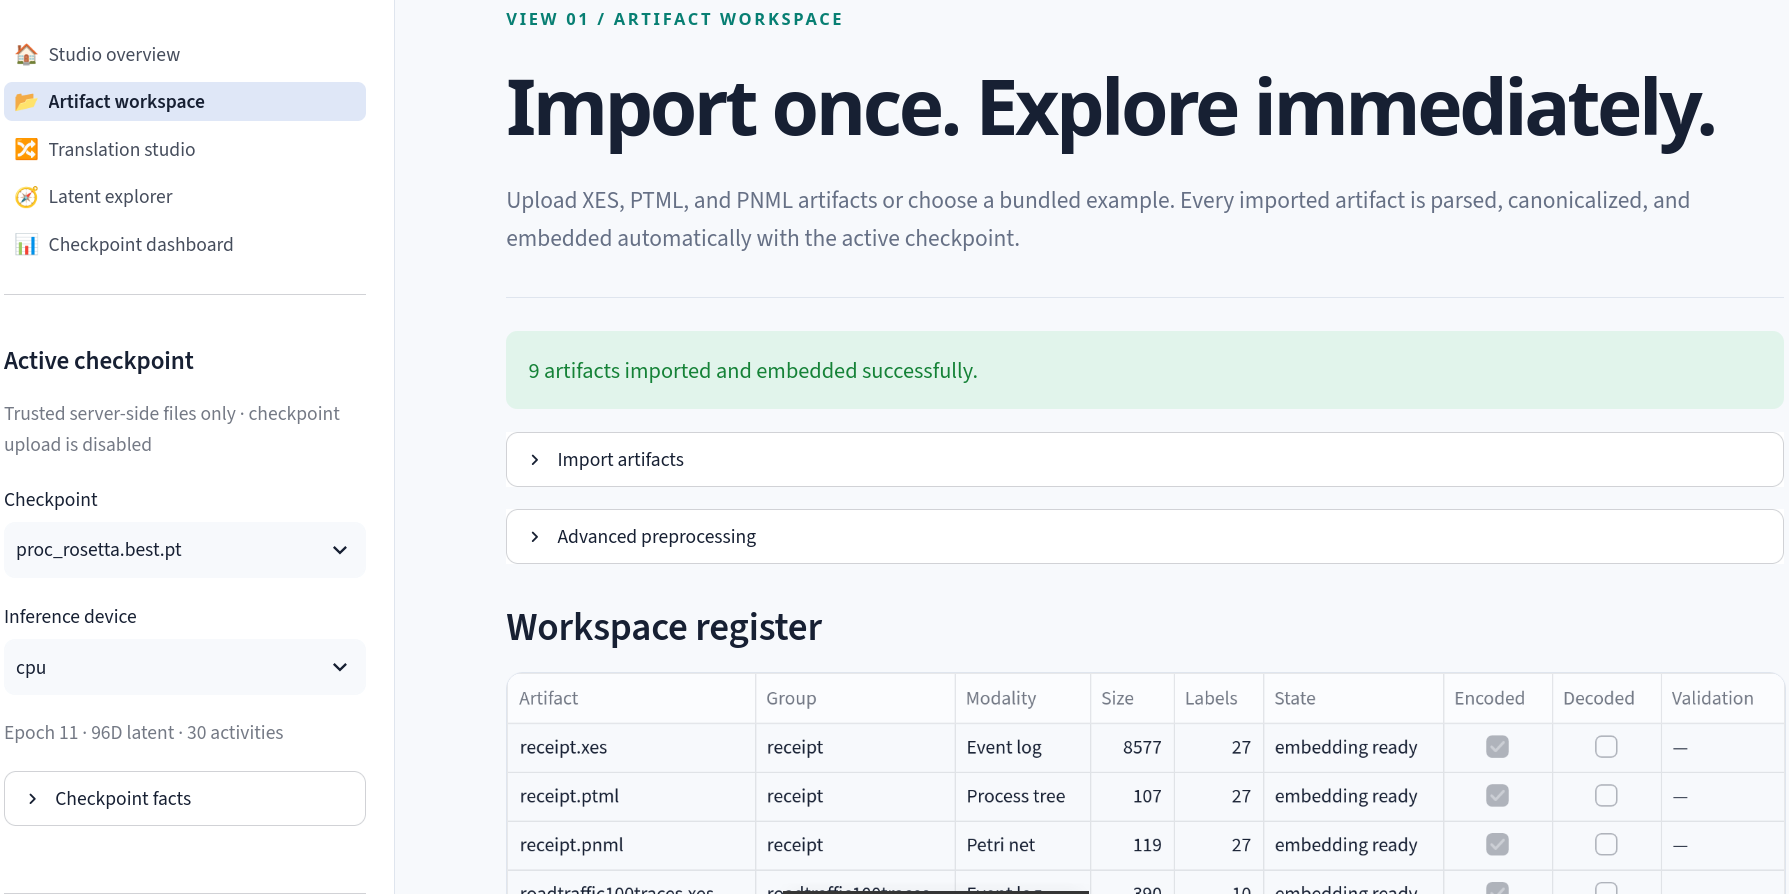
\includegraphics[width=0.90\textwidth]{screenshots/rosetta-pm-artifact-workspace.png}
\caption{Artifact workspace. The interface groups heterogeneous inputs, previews their contents, and records canonicalization and checkpoint information before encoding.\label{fig:tool-workspace}}
\end{figure*}

\paragraph{Translation studio.}
The second question is, ``What process tree does this evidence support?'' The analyst can decode one registered embedding or the equal-weight mean of the available modalities in a process group. Before decoding, the interface makes the operational constraints visible, including the token budget, restriction to the source activity alphabet, and optional masking of repeated visible labels. After decoding, it reports grammar and conversion checks and provides process tree, Petri net, and textual views. The candidate and its validation information can be exported in standard formats. Figure~\ref{fig:tool-translation} illustrates these controls. They make a proposed model easier to inspect, but they do not replace the semantic checks in Figure~\ref{fig:application-workflow}.

\begin{figure*}[!t]
\centering
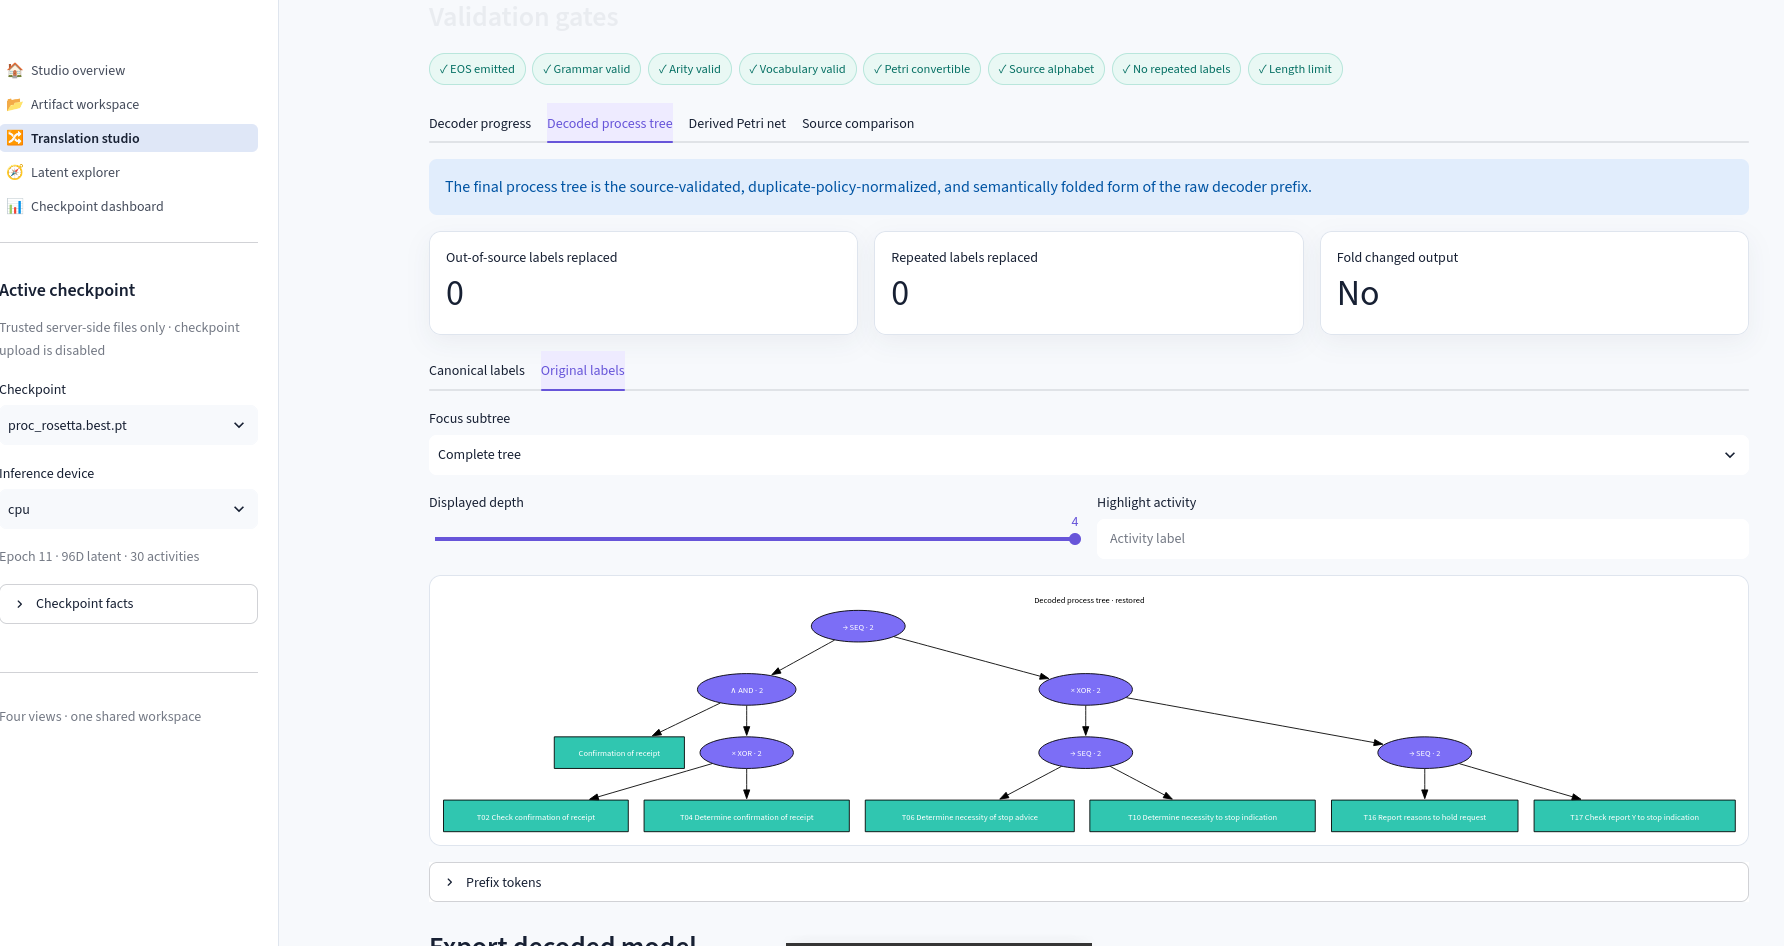
\includegraphics[width=0.88\textwidth]{screenshots/rosetta-pm-translation-studio.png}
\caption{Translation studio. An analyst selects the evidence to decode, sees the active structural constraints, and inspects and exports the resulting process model.\label{fig:tool-translation}}
\end{figure*}

\paragraph{Latent explorer.}
The third question is, ``How is this artifact related to the rest of the workspace?'' The explorer computes pairwise cosine similarities, nearest neighbors, and group-level agreement for registered artifacts. It also offers a two-dimensional PCA projection and coordinate inspection. PCA is useful for navigation, but it is only a projection of the learned space; retrieval and the reported quantitative metrics use the full representation rather than the displayed two-dimensional coordinates. Equal-weight group means make it possible to inspect the fused representations used in the experiments. Figure~\ref{fig:tool-latent} shows the explorer.

\begin{figure*}[!t]
\centering
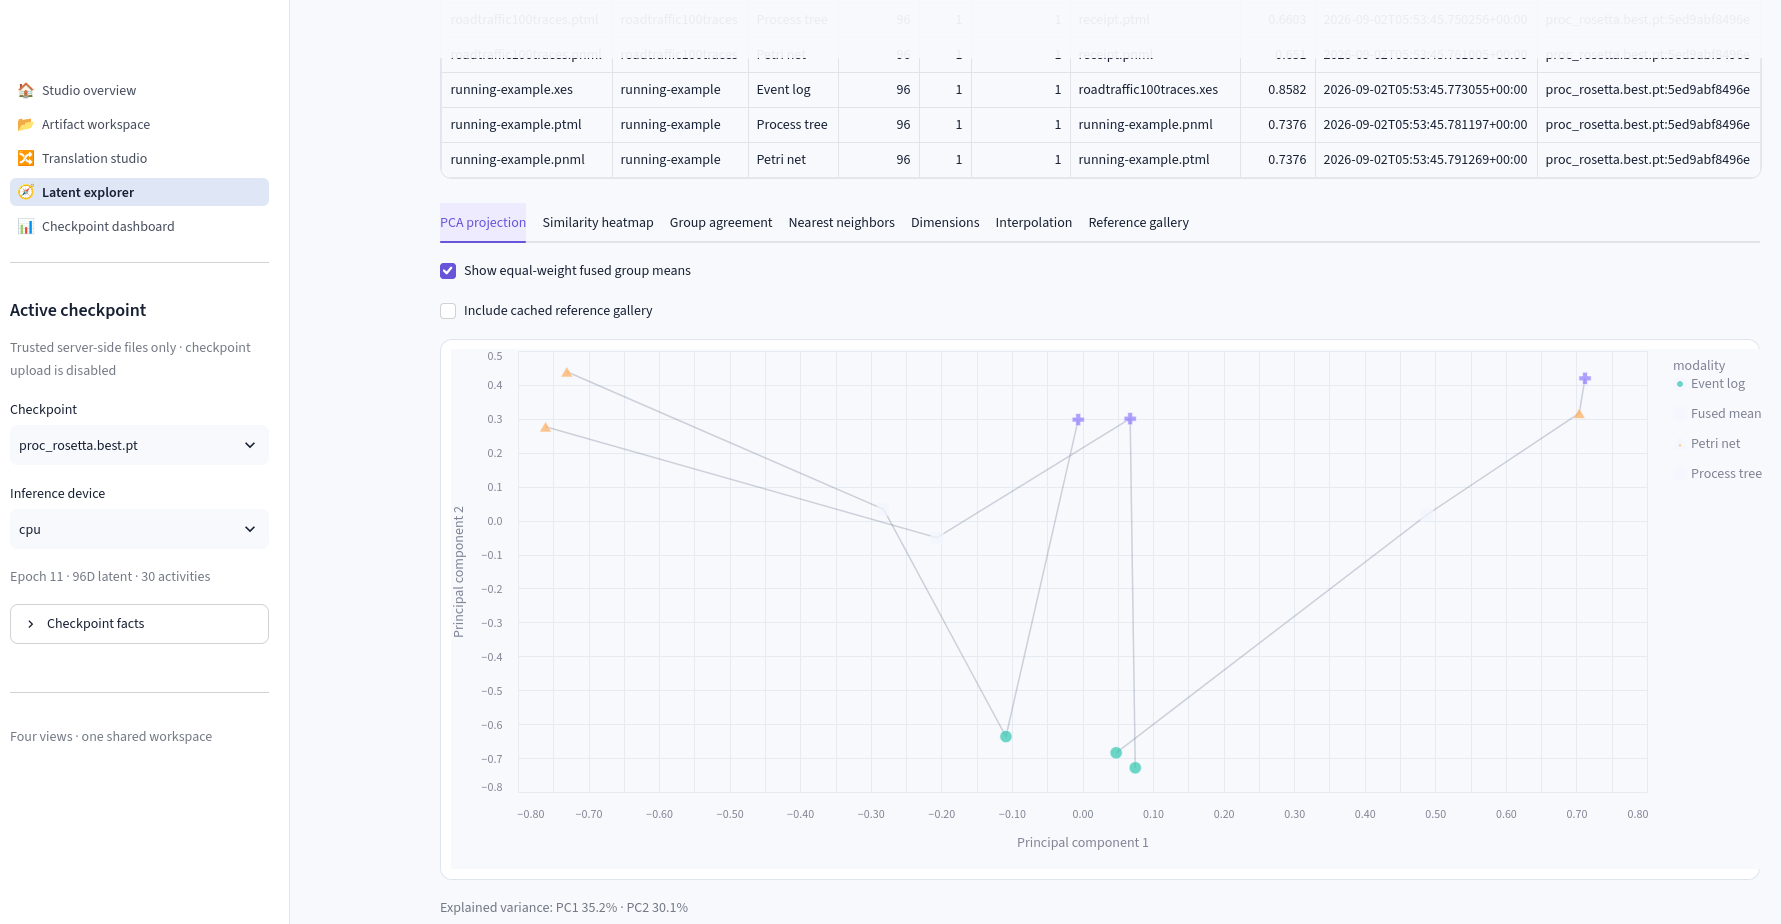
\includegraphics[width=0.88\textwidth]{screenshots/rosetta-pm-latent-explorer.png}
\caption{Latent explorer. Cosine similarities and nearest neighbors support cross-artifact inspection, while the PCA view provides an explicitly exploratory two-dimensional overview.\label{fig:tool-latent}}
\end{figure*}

The screenshots document the interaction offered by the reference implementation; they are not additional quantitative evidence. In particular, visually close points in the PCA panel and high similarity values in an individual session do not establish behavioral equivalence.

\subsection{Programmatic reproduction}

The same workflow can be executed without the browser. The following commands generate the default behavior-family corpus, train a checkpoint, evaluate one complexity level, and translate an external event log:

\begin{lstlisting}[language=bash,basicstyle=\ttfamily\footnotesize,breaklines=true,frame=single]
./sample.py --data-dir data
./train.py --data-dir data \
  --checkpoint checkpoints/proc_rosetta.pt
./test.py --data-dir data --curriculum complex \
  --checkpoint checkpoints/proc_rosetta.best.pt --json
scripts/xes_to_ptml.py input.xes decoded.ptml \
  --checkpoint checkpoints/proc_rosetta.best.pt
\end{lstlisting}

The test command evaluates exactly one of the \texttt{simple}, \texttt{medium}, or \texttt{complex} complexity levels, so it must be repeated when results for all three are required. The complete paper configuration is recorded in the curriculum manifest, the checkpoint-provenance record, and the machine-readable evaluation evidence distributed with the manuscript. These records fix the data construction, checkpoint selection, and evaluation subset instead of relying on undocumented interface state.

\FloatBarrier
\section{Results}\label{sec:results}

We report representation alignment, cross-artifact retrieval, and candidate generation using the fixed, family-complete 48-family subset in Section~\ref{sec:fixed-evaluation}. The split scope is defined in Section~\ref{sec:data-specification}; the results retain repeated observations and realizations and do not establish performance in a deduplicated repository. Discovery comparisons and external stress tests examine the limits of generation.

\subsection{\RQone: Representation alignment and behavioral ordering}

\RQone{} tests whether alternative observations and realizations remain close while distances between families reflect behavioral differences. The fused representation follows the ordering induced by $d_B$, especially at the medium and complex levels. Within-type retrieval also finds a same-family neighbor for every query, subject to the repeated-row qualification below.

\paragraph{Behavioral ordering.}
Table~\ref{tab:geometry} reports the Spearman correlation between representation distance and $d_B$, as defined in Section~\ref{sec:rq-metrics}. For fusion, it rises from 0.577 on \texttt{simple} families to 0.743 on \texttt{medium} and 0.791 on \texttt{complex}. These positive correlations indicate that greater behavioral differences generally correspond to greater representation distances, with stronger agreement at the higher levels.

\begin{table*}[!t]
\centering
\caption{Behavioral ordering on the fixed 48-family subset. Values are Spearman correlations between representation distance and $d_B$; higher positive values are better. Each level contains 16 families and 64 rows, with family pairs as the evaluation unit. Intervals use family-level bootstrap resampling for fusion.}
\label{tab:geometry}
\begin{tabular}{@{}lccc@{}}
\toprule
Representation & \texttt{simple} & \texttt{medium} & \texttt{complex} \\
\midrule
\multicolumn{4}{@{}l}{\emph{Multimodal learned representation}}\\
\model fused embedding & 0.577 & \best{0.743} & \best{0.791} \\
\quad 95\% interval & [0.405, 0.833] & [0.593, 0.868] & [0.675, 0.891] \\
\addlinespace
\multicolumn{4}{@{}l}{\emph{Single-artifact learned representations}}\\
\model event log embedding & 0.576 & 0.714 & 0.723 \\
\model Petri net embedding & 0.569 & 0.714 & 0.755 \\
\model process tree embedding & 0.433 & 0.576 & 0.680 \\
\addlinespace
\multicolumn{4}{@{}l}{\emph{Deterministic event log baselines}}\\
Trace-variant distribution & \best{0.713} & 0.628 & 0.453 \\
Directly-follows distribution & 0.550 & 0.693 & 0.750 \\
PM4Py event log features & 0.406 & 0.633 & 0.757 \\
Eventually-follows features & 0.289 & 0.503 & 0.599 \\
Activity features & 0.229 & 0.490 & 0.624 \\
\addlinespace
\multicolumn{4}{@{}l}{\emph{Deterministic Petri net baselines}}\\
Petri net count features & 0.206 & 0.562 & 0.581 \\
PM4Py Petri net Node2Vec & 0.189 & 0.201 & 0.535 \\
\bottomrule
\end{tabular}
\end{table*}

Figure~\ref{fig:geometry-bars} compares the learned representations with the deterministic baselines defined in Section~\ref{sec:rq-metrics}.

\begin{figure}[H]
\centering
\begin{tikzpicture}
\begin{axis}[
 ybar,bar width=8pt,width=0.94\textwidth,height=5.7cm,
 ymin=0,ymax=0.9,ylabel={Spearman $\rho$},
 symbolic x coords={Simple,Medium,Complex},xtick=data,
 xticklabels={\texttt{simple},\texttt{medium},\texttt{complex}},
 legend style={at={(0.5,-0.20)},anchor=north,legend columns=4,draw=none,font=\scriptsize,column sep=1.2ex},
 grid=major,grid style={prgray!15},
]
\addplot[fill=prblue,draw=prblue] coordinates {(Simple,0.577) (Medium,0.743) (Complex,0.791)};
\addplot[fill=prteal,draw=prteal] coordinates {(Simple,0.713) (Medium,0.628) (Complex,0.453)};
\addplot[fill=prgold,draw=prgold] coordinates {(Simple,0.550) (Medium,0.693) (Complex,0.750)};
\addplot[fill=prpurple,draw=prpurple] coordinates {(Simple,0.189) (Medium,0.201) (Complex,0.535)};
\legend{fused embedding,trace variants,directly follows,Petri net Node2Vec}
\end{axis}
\end{tikzpicture}
\caption{Agreement with the supervised operational behavioral distance. Higher bars are better because a larger positive Spearman $\rho$ means stronger agreement with the ordering defined by $d_B$. The fused embedding strengthens across complexity levels, while deterministic event log features remain competitive.}
\label{fig:geometry-bars}
\end{figure}


The best representation depends on process complexity. On the \texttt{simple} families, the deterministic trace-variant distribution reaches 0.713, compared with 0.577 for the fused embedding. For short synthetic processes, a small collection of complete trace variants may already describe much of the measured behavior, so a learned combination offers no advantage in this case. On the \texttt{medium} and \texttt{complex} families, the fused embedding reaches the highest value in the table. It also improves over each learned single-artifact embedding at those levels, suggesting that the combination of structural and observational information becomes more useful as the generated processes become more involved. This explanation is plausible but not established by the experiment, and the table should not be read as a significance test between individual methods.

\paragraph{Stability under alternative observations and realizations.}
Table~\ref{tab:invariance} compares alternative log observations, Petri net realizations, stored trees, and their fusion within each artifact type. The within-family cosine, between-family cosine, margin, and family Recall@1 use the definitions in Section~\ref{sec:rq-metrics}.

\begin{table*}[!t]
\centering
\caption{Stability within each artifact type on the fixed 48-family subset. Each level contains 16 families and 64 stored rows. Within and Between are the mean cosine similarities to rows from the same and different families, respectively. Margin is the nearest same-family similarity minus the nearest different-family similarity. Recall@1 is the fraction of rows whose nearest neighbor belongs to the same family. Higher Within, Margin, and Recall@1 values and lower Between values are better.}
\label{tab:invariance}
\begin{tabular}{@{}llrrrr@{}}
\toprule
Level & Encoder & Within & Between & Margin & Recall@1 \\
\midrule
\multirow{4}{*}{\texttt{simple}} & Fusion & 0.995 & 0.227 & 0.223 & 1.000 \\
 & Petri net & 0.985 & 0.220 & 0.230 & 1.000 \\
 & Event log & 0.985 & 0.316 & 0.137 & 1.000 \\
 & Process tree & 0.999 & 0.163 & 0.323 & 1.000 \\
\midrule
\multirow{4}{*}{\texttt{medium}} & Fusion & 0.993 & 0.155 & 0.287 & 1.000 \\
 & Petri net & 0.985 & 0.151 & 0.298 & 1.000 \\
 & Event log & 0.976 & 0.260 & 0.156 & 1.000 \\
 & Process tree & 0.999 & 0.118 & 0.370 & 1.000 \\
\midrule
\multirow{4}{*}{\texttt{complex}} & Fusion & 0.995 & 0.101 & 0.291 & 1.000 \\
 & Petri net & 0.985 & 0.103 & 0.326 & 1.000 \\
 & Event log & 0.982 & 0.221 & 0.182 & 1.000 \\
 & Process tree & 0.999 & 0.065 & 0.372 & 1.000 \\
\bottomrule
\end{tabular}
\end{table*}

The pattern is consistent across all three complexity levels. Within-family similarities are high, between-family similarities are substantially lower, and every reported margin is positive. Recall@1 is 1.000 in every row, meaning that the nearest neighbor always belongs to the same family under this within-type test. Process tree embeddings are the most stable, with Within values of 0.999. Event log embeddings have the smallest margins because two finite samples of the same process can contain different trace frequencies. Even so, their margins remain positive and their Recall@1 remains perfect on this subset.

\paragraph{Qualitative neighborhood examples.}
The perfect row-level Recall@1 must be read together with the two-by-two corpus expansion. Each event-log view occurs in two rows, once for each Petri net realization; likewise, each Petri realization occurs once with each log view, and the family tree is stored in all four rows. A nearest within-type row can therefore be a duplicate of the query artifact. To inspect genuinely different event-log observations, a supplementary diagnostic retained one representative per \texttt{log\_view\_id}. Each of the 32 unique \texttt{simple} log views then queried the other 31 views. The other observation from the same family ranked first for 27 of 32 queries.

Figure~\ref{fig:rq1-qualitative-retrieval} shows one of those hits and one of the five misses. For \(F_{237}\), two observations with slightly different trace frequencies have cosine similarity 0.999954 and are retrieved correctly. For \(F_{427}\), a log from \(F_{198}\) ranks first with similarity 0.962001, while the other \(F_{427}\) observation appears at rank 3 with similarity 0.937472. The cards show only selected variants for readability, but the rankings use every trace. These cases were chosen for compact presentation and are a diagnostic of the stricter distinct-view setting, not replacements for Table~\ref{tab:invariance}. Exact indices, unrounded scores, and provenance are recorded in \texttt{qualitative\_retrieval\_examples.json}.

\begin{figure*}[!t]
\centering
\resizebox{0.98\textwidth}{!}{%
\begin{tikzpicture}[
  panel/.style={draw=prgray!55,rounded corners=3pt,fill=white},
  head/.style={font=\small\bfseries,anchor=west},
  logcard/.style={
    draw=prgray!65,rounded corners=2pt,fill=prlightblue,
    align=left,font=\scriptsize,inner sep=3mm
  },
  hitcard/.style={logcard,draw=prteal,fill=prlightteal},
  misscard/.style={logcard,draw=prred,fill=prlightred},
  relevantcard/.style={logcard,draw=prgold,fill=prlightgold},
  rankarrow/.style={-{Stealth[length=2mm]},line width=0.75pt},
  score/.style={font=\scriptsize,fill=white,inner sep=1.2pt,align=center},
  verdict/.style={font=\scriptsize\bfseries,align=center}
]
% A genuine alternative-observation hit.
\node[panel,minimum width=72mm,minimum height=62mm] at (0,0) {};
\node[head] at (-3.25,2.65) {(a) Distinct-view hit};
\node[logcard,text width=57mm] (hitq) at (0,1.25) {%
  \textbf{Query log \(L_q\), \(F_{237}\)}\\[1pt]
  \(\langle A_0,A_1,A_2\rangle^{64}\)\\
  \(\langle A_0,A_2,A_1\rangle^{64}\)};
\node[hitcard,text width=57mm] (hitr) at (0,-1.15) {%
  \textbf{Top 1: other view of \(F_{237}\)}\\[1pt]
  \(\langle A_0,A_1,A_2\rangle^{60}\)\\
  \(\langle A_0,A_2,A_1\rangle^{68}\)};
\draw[rankarrow,draw=prteal] (hitq.south) -- (hitr.north)
  node[midway,right=1mm,score] {\(\cos=0.999954\)};
\node[verdict,text=prteal] at (0,-2.52)
  {HIT: the independently sampled view is ranked first};

% A genuine alternative-observation miss.
\node[panel,minimum width=103mm,minimum height=62mm] at (9.0,0) {};
\node[head] at (4.20,2.65) {(b) Distinct-view miss};
\node[logcard,text width=79mm] (missq) at (9.0,1.45) {%
  \textbf{Query log \(L_q\), \(F_{427}\)}\quad
  \(\langle A_3\rangle^{19}\),\
  \(\langle A_0,A_1,A_4\rangle^{19}\),\
  \(\langle A_0,A_1,A_2\rangle^{18}\),\ \(\ldots\) (7 variants)};
\node[misscard,text width=39mm] (wrong) at (6.55,-1.05) {%
  \textbf{Top 1: \(F_{198}\)}\\[1pt]
  \(\langle A_0,A_1,A_2\rangle^{24}\)\\
  \(\langle A_1,A_2,A_0\rangle^{19}\)\\
  \(\langle A_5,A_4\rangle^{16}\)\\
  \(\ldots\) (9 variants)};
\node[relevantcard,text width=39mm] (right) at (11.45,-1.05) {%
  \textbf{First relevant: \(F_{427}\), rank 3}\\[1pt]
  \(\langle A_3\rangle^{24}\)\\
  \(\langle A_1,A_0,A_2\rangle^{23}\)\\
  \(\langle A_0,A_1,A_2\rangle^{19}\)\\
  \(\ldots\) (7 variants)};
\draw[rankarrow,draw=prred] (missq.south west) -- (wrong.north)
  node[pos=0.62,left=1mm,score] {Top 1\\\(\cos=0.962001\)};
\draw[rankarrow,draw=prgold] (missq.south east) -- (right.north)
  node[pos=0.62,right=1mm,score] {Rank 3\\\(\cos=0.937472\)};
\node[verdict,text=prred] at (9.0,-2.52)
  {MISS: a different family is closer than the other observation};
\end{tikzpicture}%
}
\caption{Qualitative RQ1 event-log neighborhood examples from the \texttt{simple} subset, where \(F_k\) denotes family index \(k\) in that test split. One representative per \texttt{log\_view\_id} is retained, and the query itself is excluded, so every query searches 31 genuinely distinct event logs. Superscripts give trace frequencies; the complete 128-trace logs, not only the displayed variants, are embedded. In panel~(b), the relevant view's canonical labels are mapped into the query's label convention for display only.}
\label{fig:rq1-qualitative-retrieval}
\end{figure*}


\paragraph{Interpretation.}
Taken together, the results support RQ1 within the stated synthetic evaluation setting. Alternative observations and realizations remain close to their families, while distances between families reflect the ordering defined by $d_B$. This makes the representation suitable for neighborhood inspection and motivates the cross-artifact retrieval experiment in RQ2.

This ordering remains specific to $d_B$, whose semantic limits and overlap with training descriptors are described in Section~\ref{sec:rq-metrics}. Retrieval and footprint conformance provide complementary evidence without reusing this exact scalar target.

\FloatBarrier
\subsection{\RQtwo: Cross-Artifact Retrieval}\label{sec:retrieval-results}

\RQtwo{} evaluates all six ordered query-to-candidate directions among event logs, process trees, and Petri nets. Each level uses 64 candidate rows from 16 families under the relevance rule in Section~\ref{sec:rq-metrics}. Table~\ref{tab:retrieval} reports Recall@1 and MRR; higher values are better for both, and random Recall@1 is 0.0625. The results describe retrieval among stored observations and realizations, with four relevant rows per query.

\begin{table*}[!b]
\caption{Cross-artifact retrieval on the fixed 48-family subset, reported as Recall@1 / MRR. The slash is a separator, not division: the value on its left is Recall@1 and the value on its right is MRR. Higher values are better for both metrics. Each level contains 16 families and a 64-row candidate set. For every query row, all four rows from its behavior family are relevant.\label{tab:retrieval}}
\centering
\begin{tabular}{@{}lccc@{}}
\toprule
Direction & \texttt{simple} & \texttt{medium} & \texttt{complex} \\
\midrule
Petri net $\rightarrow$ event log  & 0.703 / 0.755 & 0.766 / 0.799 & 0.828 / 0.855 \\
Petri net $\rightarrow$ process tree & 0.828 / 0.862 & 0.828 / 0.862 & 0.828 / 0.862 \\
Event log $\rightarrow$ Petri net  & 0.750 / 0.805 & 0.719 / 0.785 & 0.750 / 0.801 \\
Event log $\rightarrow$ process tree & 0.656 / 0.705 & 0.656 / 0.705 & 0.688 / 0.730 \\
Process tree $\rightarrow$ Petri net & 0.812 / 0.867 & 0.875 / 0.908 & 0.875 / 0.908 \\
Process tree $\rightarrow$ event log & 0.875 / 0.905 & 0.875 / 0.905 & 0.875 / 0.905 \\
\bottomrule
\end{tabular}
\end{table*}

\paragraph{Retrieval results.}
Every tested direction is well above the random Recall@1 baseline. Recall@1 ranges from 0.656 to 0.875, compared with 0.0625 for random group selection. Thus, the shared representation contains substantial information about behavior-family membership even when the query and candidate use different artifact types. The values are not perfect, however. A Recall@1 of 0.656 means that the first result is relevant for 65.6\% of queries and incorrect for the remaining 34.4\%.

The strongest direction is process tree $\rightarrow$ event log, with Recall@1 of 0.875 and MRR of 0.905 at every complexity level. Process tree $\rightarrow$ Petri net is also strong: Recall@1 increases from 0.812 to 0.875 and MRR increases from 0.867 to 0.908 between the \texttt{simple} level and the two higher levels. These results mean that process tree queries usually place a related model or observation first and, when they do not, a relevant result still tends to appear near the top.

The most difficult direction is event log $\rightarrow$ process tree. Its Recall@1 is 0.656 on the \texttt{simple} and \texttt{medium} families and 0.688 on the \texttt{complex} families. This difficulty is consistent with the information available in the artifacts: an event log contains only finite observed executions, whereas a process tree explicitly describes control-flow structure and may permit behavior absent from the log. The experiment does not isolate this as the only cause, but it explains why this direction is intrinsically less direct.

The direction of retrieval matters. For Petri net $\rightarrow$ event log, Recall@1 increases from 0.703 to 0.828 and MRR increases from 0.755 to 0.855 across the three levels. Event log $\rightarrow$ Petri net, in contrast, remains between 0.72 and 0.75 Recall@1. This asymmetry does not contradict the use of cosine similarity: the similarity of one specific pair is symmetric, but reversing a retrieval task changes which artifacts act as queries and which collection is ranked. The two directions can therefore produce different aggregate results.

\paragraph{Qualitative retrieval examples.}
Figure~\ref{fig:rq2-qualitative-retrieval} instantiates the two possible Recall@1 outcomes for event log $\rightarrow$ process tree retrieval on the \texttt{simple} subset. The \(F_{237}\) query contains the two orders produced when \(A_1\) and \(A_2\) execute in parallel after \(A_0\). Its matching tree is ranked first with cosine similarity 0.530934. In the unsuccessful \(F_{254}\) query, all four rows from \(F_{320}\) precede every relevant row: the top similarity is 0.429963, and the first \(F_{254}\) tree appears at rank 5 with similarity 0.400794. Thus the ranking error is small in score but decisive for Recall@1, and row multiplicity makes one family-level confusion occupy four consecutive ranks. The examples were selected from the actual ranking for low visual complexity; they use the same relevance rule and candidate set as Table~\ref{tab:retrieval}.

\begin{figure*}[!t]
\centering
\resizebox{0.98\textwidth}{!}{%
\begin{tikzpicture}[
  panel/.style={draw=prgray!55,rounded corners=3pt,fill=white},
  head/.style={font=\small\bfseries,anchor=west},
  logcard/.style={
    draw=prblue,rounded corners=2pt,fill=prlightblue,
    align=left,font=\scriptsize,inner sep=3mm
  },
  candidate/.style={draw=prgray!55,rounded corners=2pt,fill=white},
  goodcandidate/.style={candidate,draw=prteal,fill=prlightteal},
  badcandidate/.style={candidate,draw=prred,fill=prlightred},
  relevantcandidate/.style={candidate,draw=prgold,fill=prlightgold},
  op/.style={
    circle,draw=prgray!75,fill=prlightgold,minimum size=5.4mm,
    inner sep=0pt,font=\scriptsize\bfseries
  },
  leaf/.style={
    rectangle,rounded corners=1pt,draw=prgray!70,fill=white,
    minimum width=7mm,minimum height=4.8mm,inner sep=1pt,font=\scriptsize
  },
  edge/.style={draw=prgray!75,line width=0.55pt},
  rankarrow/.style={-{Stealth[length=2mm]},line width=0.8pt},
  score/.style={font=\scriptsize,fill=white,inner sep=1.2pt,align=center},
  result/.style={font=\scriptsize\bfseries,align=center}
]
% Successful log-to-tree retrieval.
\node[panel,minimum width=172mm,minimum height=37mm] at (0,3.0) {};
\node[head] at (-8.15,4.42) {(a) Event log \(\rightarrow\) process tree: hit};
\node[logcard,text width=43mm] (sq) at (-5.65,2.85) {%
  \textbf{Query log, \(F_{237}\)}\\[1pt]
  \(\langle A_0,A_1,A_2\rangle^{64}\)\\
  \(\langle A_0,A_2,A_1\rangle^{64}\)};
\node[goodcandidate,minimum width=48mm,minimum height=28mm] (sg) at (0.35,2.82) {};
\node[font=\scriptsize\bfseries,text=prteal] at (0.35,3.88)
  {Top 1: relevant \(F_{237}\), \(\cos=0.530934\)};
\node[op] (sseq) at (0.35,3.25) {\(\rightarrow\)};
\node[leaf] (sa0) at (-0.55,2.45) {\(A_0\)};
\node[op] (sand) at (1.25,2.45) {\(\wedge\)};
\node[leaf] (sa1) at (0.82,1.82) {\(A_1\)};
\node[leaf] (sa2) at (1.68,1.82) {\(A_2\)};
\draw[edge] (sseq)--(sa0); \draw[edge] (sseq)--(sand);
\draw[edge] (sand)--(sa1); \draw[edge] (sand)--(sa2);
\draw[rankarrow,draw=prteal] (sq.east) -- (sg.west)
  node[midway,above=1mm,score] {rank 1};
\node[result,text=prteal] at (5.75,2.85)
  {HIT\\the first four rows are relevant};

% Unsuccessful log-to-tree retrieval.
\node[panel,minimum width=172mm,minimum height=57mm] at (0,-1.65) {};
\node[head] at (-8.15,0.60) {(b) Event log \(\rightarrow\) process tree: miss};
\node[logcard,text width=37mm] (fq) at (-6.15,-1.60) {%
  \textbf{Query log, \(F_{254}\)}\\[1pt]
  \(\langle A_0,A_2,A_1,A_3\rangle^{43}\)\\
  \(\langle A_0,A_4,A_3\rangle^{43}\)\\
  \(\langle A_0,A_1,A_2,A_3\rangle^{42}\)};

\node[badcandidate,minimum width=50mm,minimum height=44mm] (fbad) at (-1.45,-1.72) {};
\node[font=\scriptsize\bfseries,text=prred] at (-1.45,0.02)
  {Top 1: non-relevant \(F_{320}\), \(\cos=0.429963\)};
\node[op] (bseq) at (-1.45,-0.62) {\(\rightarrow\)};
\node[op] (bx1) at (-2.95,-1.38) {\(\times\)};
\node[leaf] (ba2) at (-1.45,-1.38) {\(A_2\)};
\node[op] (bx2) at (0.05,-1.38) {\(\times\)};
\node[leaf] (ba5) at (-3.55,-2.25) {\(A_5\)};
\node[op] (band) at (-2.45,-2.25) {\(\wedge\)};
\node[leaf] (ba0) at (-2.88,-3.13) {\(A_0\)};
\node[leaf] (ba1) at (-2.02,-3.13) {\(A_1\)};
\node[leaf] (ba3) at (-0.38,-2.25) {\(A_3\)};
\node[leaf] (ba4) at (0.48,-2.25) {\(A_4\)};
\draw[edge] (bseq)--(bx1); \draw[edge] (bseq)--(ba2); \draw[edge] (bseq)--(bx2);
\draw[edge] (bx1)--(ba5); \draw[edge] (bx1)--(band);
\draw[edge] (band)--(ba0); \draw[edge] (band)--(ba1);
\draw[edge] (bx2)--(ba3); \draw[edge] (bx2)--(ba4);

\node[relevantcandidate,minimum width=50mm,minimum height=44mm] (fgood) at (5.15,-1.72) {};
\node[font=\scriptsize\bfseries,text=prgold] at (5.15,0.02)
  {First relevant \(F_{254}\): rank 5, \(\cos=0.400794\)};
\node[op] (gseq) at (5.15,-0.62) {\(\rightarrow\)};
\node[leaf] (ga0) at (3.70,-1.38) {\(A_0\)};
\node[op] (gx) at (5.15,-1.38) {\(\times\)};
\node[leaf] (ga3) at (6.60,-1.38) {\(A_3\)};
\node[leaf] (ga4) at (4.55,-2.25) {\(A_4\)};
\node[op] (gand) at (5.75,-2.25) {\(\wedge\)};
\node[leaf] (ga1) at (5.32,-3.13) {\(A_1\)};
\node[leaf] (ga2) at (6.18,-3.13) {\(A_2\)};
\draw[edge] (gseq)--(ga0); \draw[edge] (gseq)--(gx); \draw[edge] (gseq)--(ga3);
\draw[edge] (gx)--(ga4); \draw[edge] (gx)--(gand);
\draw[edge] (gand)--(ga1); \draw[edge] (gand)--(ga2);

\draw[rankarrow,draw=prred] (fq.east) -- (fbad.west)
  node[midway,above=1mm,score] {rank 1};
\draw[rankarrow,draw=prgold,densely dashed] (fbad.east) -- (fgood.west)
  node[midway,above=1mm,score] {three more rows\\then rank 5};
\end{tikzpicture}%
}
\caption{Qualitative RQ2 log-to-tree retrieval examples from the reported 64-row \texttt{simple} protocol, where \(F_k\) denotes family index \(k\) in that test split. Panel~(a) is a hit: the two observed interleavings retrieve the matching sequential-then-parallel process tree. Panel~(b) is a miss: all four rows of \(F_{320}\) precede the first relevant row of \(F_{254}\). Tree nodes \(\rightarrow\), \(\times\), and \(\wedge\) denote sequence, choice, and parallelism. Rankings and cosine scores use the complete 96-dimensional vectors and all candidates. The rank-5 tree is relabeled into the query's view-local activity convention for display only.}
\Description{Two event-log-to-process-tree retrieval examples. The successful query retrieves a matching tree with a sequence followed by two parallel activities. The unsuccessful query retrieves a different family first; a tree from the correct family appears at rank five.}
\label{fig:rq2-qualitative-retrieval}
\end{figure*}


\paragraph{Two-dimensional illustration.}
Figure~\ref{fig:pca} gives an intuitive view of the cross-artifact neighborhoods behind the numerical results. Each connected set contains the event log, Petri net, and process tree representations of one behavior family. When the three markers are close, the visualization suggests that the encoders place the different artifact types in a similar region of the shared space. This is the relationship needed to retrieve one artifact type by using another as the query.

\begin{figure}[H]
\centering
\begin{tikzpicture}
\begin{axis}[
 width=0.94\textwidth,height=6.8cm,
 xlabel={PC1 (25.4\%)},ylabel={PC2 (15.0\%)},
 xmin=-1.15,xmax=0.78,ymin=-0.78,ymax=0.72,
 grid=major,grid style={prgray!12},
 legend style={at={(0.5,-0.18)},anchor=north,legend columns=3,draw=none,font=\scriptsize,column sep=1.2ex},
]
% family connectors
\foreach \xa/\ya/\xb/\yb/\xc/\yc in {
-0.150/-0.454/-0.195/-0.662/-0.028/-0.671,
0.430/0.037/0.592/-0.221/0.380/-0.231,
0.485/0.206/0.642/0.101/0.560/0.210,
0.236/0.492/0.357/0.546/0.069/0.589,
-0.711/0.147/-0.511/-0.168/-0.631/-0.333,
0.492/0.200/0.620/0.057/0.585/0.080,
0.506/0.049/0.525/-0.332/0.311/-0.507,
-0.816/0.266/-1.017/0.423/-0.974/0.437,
-0.393/-0.207/-0.354/0.120/-0.459/-0.142,
0.226/0.534/0.048/0.588/0.141/0.509,
0.058/-0.233/-0.011/-0.576/0.109/-0.572,
-0.390/-0.122/-0.376/-0.068/-0.358/-0.091}{
  \addplot[prgray!35,thin,no marks,forget plot] coordinates {(
  \xa,\ya) (\xb,\yb) (\xc,\yc) (\xa,\ya)};
}
\addplot[only marks,mark=*,mark size=2.4pt,prblue] coordinates {
(-0.150,-0.454) (0.430,0.037) (0.485,0.206) (0.236,0.492) (-0.711,0.147) (0.492,0.200)
(0.506,0.049) (-0.816,0.266) (-0.393,-0.207) (0.226,0.534) (0.058,-0.233) (-0.390,-0.122)};
\addlegendentry{event log}
\addplot[only marks,mark=square*,mark size=2.3pt,prteal] coordinates {
(-0.195,-0.662) (0.592,-0.221) (0.642,0.101) (0.357,0.546) (-0.511,-0.168) (0.620,0.057)
(0.525,-0.332) (-1.017,0.423) (-0.354,0.120) (0.048,0.588) (-0.011,-0.576) (-0.376,-0.068)};
\addlegendentry{Petri net}
\addplot[only marks,mark=triangle*,mark size=2.7pt,prgold] coordinates {
(-0.028,-0.671) (0.380,-0.231) (0.560,0.210) (0.069,0.589) (-0.631,-0.333) (0.585,0.080)
(0.311,-0.507) (-0.974,0.437) (-0.459,-0.142) (0.141,0.509) (0.109,-0.572) (-0.358,-0.091)};
\addlegendentry{process tree}
\end{axis}
\end{tikzpicture}
\caption{Joint PCA of event log, Petri net, and process tree embeddings for 12 complex families. Gray triangles connect modalities of one family. PCA is illustrative; all reported retrieval and distance results use the original 96-dimensional vectors.}
\label{fig:pca}
\end{figure}


The PCA view is only an illustration. It compresses the learned vectors to two dimensions and therefore loses information and can distort distances. The Recall@1 and MRR values in Table~\ref{tab:retrieval} are computed from the full 96-dimensional semantic vectors, not from the positions shown in Figure~\ref{fig:pca}. The figure helps explain the retrieval setting, but it is not additional quantitative evidence of retrieval quality.

\paragraph{Interpretation and scope.}
The results support RQ2 under the evaluated protocol: artifacts from the same behavior family can often be retrieved across artifact types, and the first relevant result is usually at or near the top of the ranking. This supports using the shared representation to suggest related artifacts for analyst inspection.

The scope of this conclusion is limited by the candidate set. Each relevance group contains four candidate rows, so a query has several positive observations or realizations that it can retrieve. This makes the task easier than searching a repository containing one deduplicated artifact per process. Equal multiplicity keeps the random family prior at $1/16$, but repeated rows can still affect ranks and the deterministic ordering of ties. The results must therefore be described as \emph{multi-observation retrieval}, not as deduplicated process-level retrieval.

The evaluation also uses a fixed subset generated by the same corpus design as the training data. It does not measure retrieval from a large external repository, and it does not show that the top-ranked artifact is behaviorally equivalent to a new production query. In the intended application, retrieved artifacts remain candidates that require behavioral checking and analyst review.

\subsection{\RQthree: Structural Guarantees and Behavioral Limits of Candidate Generation}\label{sec:decode-results}

\RQthree{} separates structural admissibility from behavioral fidelity. Every evaluated output is a closed process tree over the permitted vocabulary and converts to a Petri net, consistent with the conditional guarantees in Section~\ref{sec:decoder-guarantees}. These checks do not establish agreement with the source.

Table~\ref{tab:decode} compares the four source conditions in Section~\ref{sec:fixed-evaluation}. Process tree input tests reconstruction, while event log, Petri net, and fused inputs test cross-artifact generation. Higher simulation coverage and exact match are better; lower $d_B$ and tree edit distance indicate closer agreement. Mean $d_B$ includes only successfully simulated candidates, so it must be read with coverage.

\begin{table*}[!b]
\centering
\caption{Candidate-generation results on the fixed 48-family subset. Each level contains 16 families and 64 row-level source instances per source condition. Evaluable is the percentage of candidates for which behavioral simulation completed, and Exact is the percentage that equals the folded reference tree; higher values are better for both. The behavior distance $d_B$ and normalized process tree edit distance measure behavioral and structural disagreement, respectively; lower values are better. Mean $d_B$ includes only candidates for which behavioral simulation completed.}
\label{tab:decode}
\begin{tabular}{@{}llrrrr@{}}
\toprule
Level & Source & Evaluable (\%) & Exact (\%) & $d_B$ $\downarrow$ & Process tree edit $\downarrow$ \\
\midrule
\multirow{4}{*}{\texttt{simple}}
 & Process tree & 100.0 & 34.4 & 0.861 & 0.509 \\
 & Event log    & 100.0 & 0.0  & 1.169 & 0.519 \\
 & Petri net    & 100.0 & 12.5 & 1.094 & 0.661 \\
 & Fusion       & 100.0 & 3.1  & 1.148 & 0.589 \\
\midrule
\multirow{4}{*}{\texttt{medium}}
 & Process tree & 100.0 & 28.1 & 0.950 & 0.549 \\
 & Event log    & 96.9  & 0.0  & 1.246 & 0.553 \\
 & Petri net    & 100.0 & 6.2  & 1.130 & 0.645 \\
 & Fusion       & 100.0 & 0.0  & 1.222 & 0.668 \\
\midrule
\multirow{4}{*}{\texttt{complex}}
 & Process tree & 100.0 & 15.6 & 1.105 & 0.645 \\
 & Event log    & 100.0 & 0.0  & 1.291 & 0.562 \\
 & Petri net    & 100.0 & 6.2  & 1.245 & 0.673 \\
 & Fusion       & 93.8  & 0.0  & 1.273 & 0.676 \\
\bottomrule
\end{tabular}
\end{table*}

\paragraph{Results by source artifact.}
Process tree input gives the best overall reconstruction results. This is expected because the source already has the same hierarchical structure as the output. Even in this favorable condition, however, exact match falls from 34.4\% for \texttt{simple} families to 28.1\% for \texttt{medium} families and 15.6\% for \texttt{complex} families. At the same time, $d_B$ increases from 0.861 to 1.105 and tree-edit distance increases from 0.509 to 0.645. Because lower distances are better, both trends show that reconstruction becomes less faithful as process complexity increases.

Event log input is the hardest condition. Its exact-match rate is 0\% at every level, and its behavioral distance increases from 1.169 to 1.291. An event log does not expose an explicit control-flow hierarchy and contains only the executions that happened to be sampled, so the decoder must infer choices, concurrency, loops, and unobserved paths. A zero exact-match rate is not sufficient by itself to prove behavioral failure, because several different process trees may legitimately explain the same finite log. In this experiment, however, the relatively large $d_B$ values show that the differences are not only harmless alternative tree structures.

Petri net input performs between process tree and event log input for exact reconstruction. It reaches 12.5\% exact match on \texttt{simple} families and 6.2\% on the two higher levels. The Petri net contains explicit control-flow structure, but that structure must still be converted from a graph into the hierarchical organization required by a process tree. The edit and behavior distances show that this conversion remains difficult even though every output is grammatically valid.

Equal-weight fusion does not improve on the strongest individual source. It reaches 3.1\% exact match on \texttt{simple} families and 0\% on the other levels, while its $d_B$ is higher than that of the best individual source at every level. This result suggests that a simple average can discard useful source-specific information or give equal influence to sources of unequal reliability. The present experiment evaluates the stated equal-weight policy only; it does not establish that every learned or reliability-aware fusion method would behave in the same way.

Evaluator coverage is close to complete but must still be reported. Most conditions reach 100\%. The exceptions are event log input on \texttt{medium} families, with 96.9\%, and fusion on \texttt{complex} families, with 93.8\%. These missing evaluations arise when a grammar-valid candidate becomes too large for reliable behavioral simulation within the evaluation safeguards. This again illustrates the main distinction of RQ3: a tree may satisfy every structural rule and still be difficult to evaluate or behaviorally unsuitable.

\paragraph{Where the decoding errors occur.}
Table~\ref{tab:motif-decode} separates event-log decoding by generator family type, using behavioral and structural distance to show where errors are concentrated.

The three controlled motifs remain small and have the same designed structure at every complexity level. Their nearly unchanged values should therefore not be interpreted as evidence that decoding is unaffected by complexity. They are fixed diagnostic cases. The ordinary families, in contrast, become larger and deeper across complexity levels and may contain more demanding nested or looping behavior. Their $d_B$ rises from 1.224 to 1.715, while their edit distance rises from 0.662 to 0.832. These increases localize the strongest degradation in the families whose structural complexity actually grows.

\begin{table*}[!b]
\centering
\caption{Event log to process tree decoding by family type on the fixed 48-family subset. Each cell reports $d_B$ / normalized process tree edit distance. The slash is a separator, not division: $d_B$ is on the left and tree-edit distance is on the right. Lower values are better for both quantities. Each level contains 16 families and 64 event log source rows, including repeated observations.}
\label{tab:motif-decode}
\begin{tabular}{@{}lccc@{}}
\toprule
Family type & \texttt{simple} & \texttt{medium} & \texttt{complex} \\
\midrule
Duplicate prefix & 1.136 / 0.546 & 1.187 / 0.546 & 1.165 / 0.546 \\
Concurrency/interleaving & 1.087 / 0.491 & 1.081 / 0.491 & 1.063 / 0.491 \\
M-pattern & 1.175 / 0.378 & 1.170 / 0.378 & 1.130 / 0.378 \\
Ordinary & 1.224 / 0.662 & 1.580 / 0.798 & 1.715 / 0.832 \\
\bottomrule
\end{tabular}
\end{table*}

\paragraph{Interpretation and scope.}
The answer to RQ3 is therefore mixed but clear. The grammar constraints provide the promised \emph{structural guarantee}: every decoded output is a closed process tree over the permitted vocabulary and is convertible to a Petri net. They do not provide a \emph{behavior-preservation guarantee}. Exact reconstruction is limited, behavioral disagreement grows with ordinary-family complexity, and equal-weight fusion does not repair the problem.

The decoder should consequently be used as a candidate generator rather than as an automatic translator. Its output is structurally usable, which makes subsequent analysis possible, but the candidate must still undergo conformance checking, soundness analysis, and human inspection before acceptance. The next subsection makes this practical limitation more concrete by comparing event log decoding with a specialized process discovery method.

\subsection{Comparison with Specialized Process Discovery}

To assess the practical value of candidate generation from event logs, we compare its behavioral fidelity with a method designed specifically for process discovery.

Table~\ref{tab:discovery} compares event log decoding with Inductive Miner. \model remains substantially below the specialized method on footprint F1 and has lower footprint-evaluator coverage. The strong Inductive Miner results are consistent with the favorable experimental setting: the event logs are clean and much of the synthetic corpus originates from block-structured process trees. The comparison nevertheless answers the practical question posed by \RQthree: whether \model currently improves process discovery from event logs into process trees under the conditions in which it was trained. It does not.

\begin{table*}[!b]
\centering
\caption{Process discovery from event logs on the fixed 48-family detailed subset using 64 event log source rows per level (16 families; repeated observations retained; no retrieval candidate set). The evaluation unit is a discovered model. Higher fitness, precision, and F1 values are better; evaluable is the percentage for which the footprint routine completed. Intervals are family-bootstrap intervals for F1.}
\label{tab:discovery}
\setlength{\tabcolsep}{4pt}
\begin{tabular}{@{}llrrrrl@{}}
\toprule
Level & Method & Evaluable (\%) & Fitness & Precision & F1 & 95\% interval \\
\midrule
\multirow{2}{*}{\texttt{simple}}
 & \model{} & 78.1 & 0.702 & 0.654 & 0.666 & [0.598, 0.746] \\
 & Inductive Miner & 100.0 & 1.000 & 0.992 & 0.996 & [0.987, 1.000] \\
\midrule
\multirow{2}{*}{\texttt{medium}}
 & \model{} & 75.0 & 0.709 & 0.663 & 0.669 & [0.611, 0.733] \\
 & Inductive Miner & 100.0 & 1.000 & 0.986 & 0.992 & [0.975, 1.000] \\
\midrule
\multirow{2}{*}{\texttt{complex}}
 & \model{} & 71.9 & 0.691 & 0.639 & 0.649 & [0.570, 0.729] \\
 & Inductive Miner & 100.0 & 1.000 & 0.907 & 0.938 & [0.868, 0.991] \\
\bottomrule
\end{tabular}
\end{table*}

\subsection{External Event Log Generation Stress Test}

The external event logs test how candidate generation behaves beyond the synthetic data, using the input-shift protocol in Section~\ref{sec:real-log-design}.

For the real event logs, the dominant failure is underfitting rather than repeated labels. The decoded receipt process tree retains only six of 27 observed activities, and the road-traffic process tree retains eight of ten. Allowing repeated labels changes neither top-ranked process tree because neither unconstrained result repeats an activity. This null result only rules out forced uniqueness as the cause of these two failures; it does not show that the policies are generally equivalent. Inductive Miner attains higher footprint F1 on both samples, although its receipt process model trades perfect fitness for relatively low precision.

\begin{table*}[!b]
\centering
\caption{External event log generation stress test for two event logs (Receipt: 128 selected cases; Road Traffic: 100 cases; no retrieval candidate set). The evaluation unit is one generated or mined model per method and event log. Higher fitness, precision, and F1 values are better. ``Repeat'' counts visible leaves beyond the first occurrence of each label.}
\label{tab:real-log-results}
\setlength{\tabcolsep}{3pt}
\begin{tabularx}{\textwidth}{@{}p{0.14\textwidth}Yrrrrr@{}}
\toprule
Event log & Method & Size & Repeat & Fitness & Precision & F1 \\
\midrule
\multirow{3}{*}{Receipt}
 & \model, duplicates allowed & 9 & 0 & 0.508 & 0.500 & 0.504 \\
 & \model, duplicates disallowed & 9 & 0 & 0.508 & 0.500 & 0.504 \\
 & Inductive Miner & 47 & 0 & 1.000 & 0.462 & \best{0.632} \\
\midrule
\multirow{3}{*}{Road traffic}
 & \model, duplicates allowed & 11 & 0 & 0.661 & 0.391 & 0.491 \\
 & \model, duplicates disallowed & 11 & 0 & 0.661 & 0.391 & 0.491 \\
 & Inductive Miner & 29 & 0 & 1.000 & 0.621 & \best{0.766} \\
\bottomrule
\end{tabularx}
\end{table*}

Figure~\ref{fig:real-log-tree} shows the road-traffic output using the process tree representation and layout supplied by PM4Py. Its compact structure makes the underfitting visible: several activities are grouped under one parallel branch, while two appeal activities are placed directly in the top-level sequence.

\begin{figure*}[!t]
\centering
\resizebox{0.86\textwidth}{!}{%
\begin{tikzpicture}[
  op/.style={circle,draw=prgray,fill=prlightgold,minimum size=6.5mm,font=\scriptsize\bfseries,inner sep=1pt},
  leaf/.style={ellipse,draw=prgray!75,fill=prlightblue,align=center,font=\scriptsize,inner sep=2.5pt},
  branch/.style={draw=prgray!75,line width=0.45pt}
]
\node[op,minimum width=1.43cm,minimum height=0.95cm] (pt0) at (6.788,6.698) {SEQ};
\node[leaf,minimum width=2.65cm,minimum height=0.95cm] (pt1) at (2.518,4.665) {Create Fine};
\node[op,minimum width=1.43cm,minimum height=0.95cm] (pt2) at (5.038,4.665) {XOR};
\node[leaf,minimum width=2.33cm,minimum height=0.95cm] (pt3) at (3.870,2.633) {Send Fine};
\node[op,minimum width=1.43cm,minimum height=0.95cm] (pt4) at (6.231,2.633) {AND};
\node[leaf,minimum width=2.65cm,minimum height=0.95cm] (pt5) at (1.324,0.600) {Add penalty};
\node[leaf,minimum width=3.11cm,minimum height=1.20cm] (pt6) at (4.693,0.600) {Insert Fine\\Notification};
\node[leaf,minimum width=2.07cm,minimum height=0.95cm] (pt7) at (7.770,0.600) {Payment};
\node[leaf,minimum width=3.86cm,minimum height=1.20cm] (pt8) at (11.218,0.600) {Send for Credit\\Collection};
\node[leaf,minimum width=4.65cm,minimum height=1.20cm] (pt9) at (8.565,4.665) {Insert Date Appeal\\to Prefecture};
\node[leaf,minimum width=3.83cm,minimum height=1.20cm] (pt10) at (13.287,4.665) {Send Appeal to\\Prefecture};
\draw[branch] (pt0) -- (pt1);
\draw[branch] (pt0) -- (pt2);
\draw[branch] (pt0) -- (pt9);
\draw[branch] (pt0) -- (pt10);
\draw[branch] (pt2) -- (pt3);
\draw[branch] (pt2) -- (pt4);
\draw[branch] (pt4) -- (pt5);
\draw[branch] (pt4) -- (pt6);
\draw[branch] (pt4) -- (pt7);
\draw[branch] (pt4) -- (pt8);
\end{tikzpicture}
}%
\caption{Road-traffic process tree decoded by \model. PM4Py supplies the process tree representation and Graphviz layout, which are emitted here as TikZ. Allowing or disallowing repeated visible labels produces this same top-ranked process tree.}
\label{fig:real-log-tree}
\end{figure*}




\section{Discussion}\label{sec:discussion}

The main question is not only whether one model can read event logs, process trees, and Petri nets, but also what it can reliably do with them. The results show a clear difference between \emph{representation} and \emph{generation}. The shared space supports cross-artifact retrieval and broadly preserves behavioral ordering. Training on behavior families helps the encoders ignore surface differences, such as two event log samples from the same process or two differently structured Petri nets that realize the same behavior. The explicit contrast between concurrency and interleaving also prevents equal visible traces from being treated automatically as complete behavioral equivalence.

This shared representation is most useful as a common search interface. For example, an event log can retrieve related process trees or Petri nets without a separate matcher for every pair of artifact types. The retrieved items can provide precedents for model reuse, variant comparison, or later conformance checking. Deterministic features nevertheless remain strong, especially for simple processes whose small observed language already describes much of their behavior. The learned representation becomes more competitive for larger structures, but its main advantage is one interface across artifact types, not the replacement of every specialized similarity measure. Moreover, the retrieval evidence comes from a controlled candidate set and does not yet establish performance in a large, deduplicated repository.

Process tree generation is less reliable. Under the conditions in Section~\ref{sec:decoder-guarantees}, the grammar guarantees a well-formed tree and the source-alphabet mask limits visible labels to the source vocabulary, but neither guarantee says that the generated tree preserves the source behavior. An incorrect operator or number of children near the start of the prefix can change the whole remaining structure. This often leads to omitted activities or overly compressed control flow. A finite event log can admit several correct models, so a generated tree need not match the chosen reference exactly; however, the lower behavioral and conformance scores show that ambiguity alone does not explain the errors. Allowing duplicate labels did not change the outputs for the two external event logs, so forced label uniqueness was not the cause of their poor results.

These findings suggest a workflow that \emph{retrieves, proposes, and validates}. The model first retrieves related artifacts, then proposes one or more process trees, and finally uses conformance checking and human review to decide whether a proposal is acceptable. Generation could be improved by producing several candidates and reranking them with behavioral evidence, training with objectives defined on complete decoded behavior, and allowing the model to report low confidence or abstain. The lack of improvement from simple mean fusion also suggests learning how much to trust each artifact type or combining their detailed source representations directly. The external event logs reveal sensitivity to inputs outside the synthetic training distribution; because they have no aligned reference artifacts in all three forms, they illustrate generation under distribution shift rather than deployment performance. The model should therefore be viewed as a retrieval and proposal tool, not as an unattended replacement for process discovery or conformance checking.

\FloatBarrier
\section{Limitations}\label{sec:threats}

The proposed retrieval and validation workflow depends on how far the experimental findings extend beyond the evaluated setting. This section examines the limits imposed by the data, output language, and evaluation design on claims about alignment, retrieval, and generation.

Most evidence comes from synthetic behavior families produced by the same generator used to create the training data. Holding out complete families prevents artifacts from one family from appearing in different splits, but independently generated families were not globally deduplicated by normalized process tree or visible language. The synthetic data also omit timestamps, resources, lifecycle information, drift, and meaningful activity names. In addition, the generator supplies relation labels that would be harder to obtain for real artifacts. The results therefore show generalization to new families from the same generator, not transfer to industrial data or to behavior that is guaranteed to be globally distinct from the training set.

The two external event logs only illustrate how generation behaves under an input shift. They have no aligned reference process trees and Petri nets, so they cannot evaluate cross-artifact retrieval. The decoder is also limited to block-structured process trees. Some Petri net behavior cannot be expressed exactly in this grammar, which means that generation error may combine model error with a limitation of the output language.

The detailed evaluation uses a fixed subset of 48 families and one checkpoint from one training seed. The bootstrap intervals capture variation among those selected families, but not variation caused by corpus generation, initialization, training, or checkpoint selection. Some behavioral averages include only cases for which evaluation succeeded, and $d_B$ partly overlaps with descriptors used during training. Finally, the baselines do not cover every discovery method or a directly comparable learned cross-artifact system, and the study does not retrain separate ablations of the architecture, family design, curriculum, fusion method, or loss terms. Stronger evidence will require real aligned artifacts, globally behavior-disjoint data, repeated runs, unconditional failure reporting, broader baselines, and retrained ablations.

\FloatBarrier
\section{Conclusion}\label{sec:conclusion}

\model demonstrates that heterogeneous process artifacts can currently be aligned more successfully than they can be translated. By training on relation-annotated behavior families, the neural system learns a common space in which event logs, process trees, and Petri nets from related families can be retrieved and compared. Grammar-constrained decoding solves a different problem: it ensures that every generated output is a well-formed process tree, but it does not ensure that the process tree preserves the source behavior.

The synthetic experiments and two real event log illustrations show that direct event log to process tree generation remains below the Inductive Miner baseline in the reported conformance checking experiments and that syntactic constraints alone do not prevent activity omission or incorrect control-flow placement. The present value of \model is therefore as a shared representation and retrieval layer that can propose candidates for subsequent validation, not as an autonomous process discovery system. The next step is to improve behavior-aware candidate generation and evaluate it on behavior-disjoint, real multi-artifact benchmarks, including structures outside the process tree grammar.

\FloatBarrier

\authorcontributions{Conceptualization and methodology, both authors; software, formal analysis, investigation, data curation, visualization, and writing (original draft preparation), A.B.; validation, supervision, and writing (review and editing), W.M.P.v.d.A. All authors have read and agreed to the published version of the manuscript.}

\funding{Funded by the European Union. This work has received funding from the EuroHPC Joint Undertaking and BMFTR, MKW NRW, and HMWK under Grant Agreement No. 101250682. Views and opinions expressed are, however, those of the authors only and do not necessarily reflect those of the European Union or the granting authorities.}

\institutionalreview{Not applicable. The study did not collect new human-subject data.}

\informedconsent{Not applicable.}

\dataavailability{Code, data, and the trained model are available at \url{https://github.com/fit-alessandro-berti/proc-rosetta}. An accompanying guide to the Streamlit interface, checked against the application source code, is provided in \path{paper_applsci/streamlit_interface_guide.tex} in the same repository. The external event logs are cited in Section~\ref{sec:real-log-design}.}

\acknowledgments{The authors thank the Process and Data Science group at RWTH Aachen University.}

\conflictsofinterest{Wil M. P. van der Aalst is affiliated with Celonis. No other competing interests are declared.}

\specialsection{Use of Generative Artificial Intelligence}{The authors used OpenAI Codex for language and LaTeX editing of the manuscript and for preparing, checking, and updating the accompanying Streamlit interface guide against the application source code. The authors reviewed the manuscript text and take full responsibility for its content.}

\reftitle{References}
\bibliography{references}

\end{document}
